% C3: Committed Confidence Calibration -- final viva slides (pass 1: structure, background, C2).
%
%   python3 documents/viva-slides/make_macros.py     # macros_setup.tex from artifacts/*.json
%   tectonic documents/viva-slides/slides.tex        # XeTeX; from the repository root
%
% Every number on a slide is a macro read from a committed artifact:
%   macros_setup.tex                    \Viva...   C1 arms, floors, design constants, 110M, probe size
%   ../../artifacts/t0/macros.tex       \TZero...  T0 simulations
%   ../../artifacts/probe/macros_t9.tex \CTwo...   T9, C2 on the JSON probe
%   ../../artifacts/c2/macros_t10.tex   \CTwoTTen... T10, C2 on real text
% Pass 2 adds the C1 report-half macros (prereg/analysis_commands.sh writes
% results/c1/<Label>/macros.tex, prefix COne<Label>) and the C3 macros (artifacts/c3/).
% Grid values (k, rho, mask rates as axis labels) are design constants, typed as the paper
% types them, with their source in a comment.
%
% Style, theme and the background slides come from documents/mid-eval-slides/slides.tex.
% Fonts are loaded by file name: tectonic core-dumps when fontspec looks one up by family.

\documentclass[aspectratio=169,10pt,t]{beamer}

\usefonttheme{professionalfonts}
\usepackage[sfdefault,lining,book,semibold]{FiraSans}
\usepackage[mathrm=sym]{unicode-math}
\setmathfont{FiraMath-Regular.otf}

\usepackage{booktabs}
\usepackage{colortbl}
\usepackage{tabularx}
\usepackage{array}
\usepackage{xspace}
\usepackage{xfp}
\usepackage{graphicx}
\usepackage{appendixnumberbeamer}
\usepackage{tikz}
\usetikzlibrary{positioning,arrows.meta,calc}
\usepackage[most]{tcolorbox}

\graphicspath{{../../artifacts/probe/figures/}{../mid-eval-slides/figures/}}

% Generated by documents/viva-slides/make_macros.py -- do not edit by hand.
% Sources (sha256):
%   artifacts/c1/c1-llada-base.json  77e6944d5807ceeaaf8d074128625ff1fe79c837c3f995f25937a690472671dd
%   artifacts/c1/c1-dream-base.json  bc7c433012431a35dbd3d2e853250706d1c09f143405b6252a2678f08b5fecf3
%   artifacts/c1/c1-llada-instruct-gsm8k.json  c83aa81bb1bfd3ce313301c828ca88a7f37eee408f3d7c8d91dc1114c04f8563
%   artifacts/c1/c1-llada-instruct-mbpp-v2.json  0285e9a86be97ce41fc0e0fe0bf4f97d7f466b7909d51c784d699ac9e84771ed
%   artifacts/c1/c1-dream-instruct-gsm8k.json  4e98ed7c2ca46a15ed133d774b8bc3cfd7bcac4e4fd3895e19495668168af2a1
%   artifacts/c1/c1-dream-instruct-mbpp.json  a1967d3841a8cb5d6d52d325ff82659914654f2e3c7d287766050060576d03be
%   artifacts/c1/main-110m-v3.json  29064b0ea911e02d43101babf1e37edfe64b4e33ac9f8ac97574dcd82cfcdea2
%   artifacts/c1/c1ts-llada-base.json  dabe6c2335b8d34e4f62324a82a88b84909bcd6153e969846e46e5a0e934e0d3
%   artifacts/c1/c1ts-dream-base.json  9d20e73df7e29714e0730a2536ef6156b53389dfbd97f0333c239dd96430e56c
%   artifacts/c1/timesplit-110m-v3.json  5fb5a5c8b3ff1afc5237d1f4225f837bec64d580ddad90227ea656111582b8b8
%   artifacts/c1/c1t8-llada-base-4bit.json  bdd60bd0a437bda491afe09275d50bff076daa9f0af23386d7b4f9e8b0ae661f
%   artifacts/t2_pilot/floor_llada_base_fp16.json  a19a8bd481b838f388ef125b184df2523556e035a24aace78ed7c2767d2cdc7f
%   artifacts/t2_pilot/floor_dream-7b-base_fp16.json  7e2eacbf1c935c9ef3e6db1071ead2f637254d572757685116af3b2802ca2dc1
%   artifacts/t2_pilot/floor_local-110m-v3_fp32.json  be8f01782e420c2e625438aace2bdc4ed6564dd27d1319c4b9ba153f42912653
%   c3/__init__.py  94bdef83e6fa785707c8b561c8b43e001f876c05b405af6bc38d71c484f8adf0
%   artifacts/split_manifest.meta.json  752d14955aeb966658ab5f10400025e7fe024bdae4da35bcb21dbcd0b19b6bce
%   artifacts/contamination_llada-8b-base.json  a55922c6bb4bfbf5af2fa988323380c07da7ed325ce3de571f859c7a94d13700
%   artifacts/contamination_dream-7b-base.json  1e60e035f07c1cebe3b64d37211dc97c5f9a467db8328f14cc212a3e145e2f9e
%   artifacts/train_summary_train110m-v3.json  b79440a6cda188d0998aff6e13a66090196eaeb4dcd2a60697ce12abdfee1308
%   artifacts/eval_110m_train110m-v3.json  e8f5094e46145a9385be559f7fed1f92def4fff7f5ec8e8247356151a70fe86b
%   artifacts/probe/manifest.json  f8194f98e0b1c3393f3e1fa80f7ae3f6adb91cc04b1fb16f60ee24d6b1fae7ca

\newcommand{\VivaLladaBaseDocs}{1{,}979}  % c1-llada-base: summary.documents
\newcommand{\VivaLladaBaseRowsM}{119.6}  % summary.rows / 1e6
\newcommand{\VivaLladaBasePasses}{922{,}214}  % summary.forward_passes
\newcommand{\VivaLladaBaseGpuH}{68}  % summary.gpu_hours
\newcommand{\VivaLladaBasePrecision}{fp16}  % summary.precision
\newcommand{\VivaDecoderK}{2, 4, 8}  % design.decoder_k
\newcommand{\VivaMaskRateMin}{0.1}  % design.mask_rates
\newcommand{\VivaMaskRateMax}{0.9}  % design.mask_rates
\newcommand{\VivaMasksPerRate}{2}  % design.masks_per_rate
\newcommand{\VivaPassesPerDoc}{466}  % checks.forward_passes.per_doc
\newcommand{\VivaCorpusDocs}{2{,}000}  % checks.every_document_present.n_corpus
\newcommand{\VivaTopK}{20}  % design.topk
\newcommand{\VivaDreamBaseDocs}{1{,}976}  % c1-dream-base: summary.documents
\newcommand{\VivaDreamBaseRowsM}{119.4}  % summary.rows / 1e6
\newcommand{\VivaDreamBasePasses}{920{,}816}  % summary.forward_passes
\newcommand{\VivaDreamBaseGpuH}{60}  % summary.gpu_hours
\newcommand{\VivaDreamBasePrecision}{fp16}  % summary.precision
\newcommand{\VivaLladaInstructGsmDocs}{1{,}319}  % c1-llada-instruct-gsm8k: summary.documents
\newcommand{\VivaLladaInstructGsmRowsM}{13.8}  % summary.rows / 1e6
\newcommand{\VivaLladaInstructGsmPasses}{245{,}152}  % summary.forward_passes
\newcommand{\VivaLladaInstructGsmGpuH}{18}  % summary.gpu_hours
\newcommand{\VivaLladaInstructGsmPrecision}{fp16}  % summary.precision
\newcommand{\VivaLladaInstructMbppDocs}{499}  % c1-llada-instruct-mbpp-v2: summary.documents
\newcommand{\VivaLladaInstructMbppRowsM}{3.1}  % summary.rows / 1e6
\newcommand{\VivaLladaInstructMbppPasses}{66{,}658}  % summary.forward_passes
\newcommand{\VivaLladaInstructMbppGpuH}{5}  % summary.gpu_hours
\newcommand{\VivaLladaInstructMbppPrecision}{fp16}  % summary.precision
\newcommand{\VivaDreamInstructGsmDocs}{1{,}319}  % c1-dream-instruct-gsm8k: summary.documents
\newcommand{\VivaDreamInstructGsmRowsM}{13.4}  % summary.rows / 1e6
\newcommand{\VivaDreamInstructGsmPasses}{241{,}162}  % summary.forward_passes
\newcommand{\VivaDreamInstructGsmGpuH}{14}  % summary.gpu_hours
\newcommand{\VivaDreamInstructGsmPrecision}{fp16}  % summary.precision
\newcommand{\VivaDreamInstructMbppDocs}{499}  % c1-dream-instruct-mbpp: summary.documents
\newcommand{\VivaDreamInstructMbppRowsM}{2.5}  % summary.rows / 1e6
\newcommand{\VivaDreamInstructMbppPasses}{60{,}680}  % summary.forward_passes
\newcommand{\VivaDreamInstructMbppGpuH}{4}  % summary.gpu_hours
\newcommand{\VivaDreamInstructMbppPrecision}{fp16}  % summary.precision
\newcommand{\VivaMdlmDocs}{1{,}979}  % main-110m-v3: summary.documents
\newcommand{\VivaMdlmRowsM}{119.6}  % summary.rows / 1e6
\newcommand{\VivaMdlmPasses}{314{,}661}  % summary.forward_passes
\newcommand{\VivaMdlmGpuH}{3}  % summary.gpu_hours
\newcommand{\VivaMdlmPrecision}{fp32}  % summary.precision
\newcommand{\VivaLladaBaseTimeSplitDocs}{500}  % c1ts-llada-base: summary.documents
\newcommand{\VivaLladaBaseTimeSplitRowsM}{30.2}  % summary.rows / 1e6
\newcommand{\VivaLladaBaseTimeSplitPasses}{233{,}000}  % summary.forward_passes
\newcommand{\VivaLladaBaseTimeSplitGpuH}{17}  % summary.gpu_hours
\newcommand{\VivaLladaBaseTimeSplitPrecision}{fp16}  % summary.precision
\newcommand{\VivaDreamBaseTimeSplitDocs}{500}  % c1ts-dream-base: summary.documents
\newcommand{\VivaDreamBaseTimeSplitRowsM}{30.2}  % summary.rows / 1e6
\newcommand{\VivaDreamBaseTimeSplitPasses}{233{,}000}  % summary.forward_passes
\newcommand{\VivaDreamBaseTimeSplitGpuH}{15}  % summary.gpu_hours
\newcommand{\VivaDreamBaseTimeSplitPrecision}{fp16}  % summary.precision
\newcommand{\VivaMdlmTimeSplitDocs}{500}  % timesplit-110m-v3: summary.documents
\newcommand{\VivaMdlmTimeSplitRowsM}{30.2}  % summary.rows / 1e6
\newcommand{\VivaMdlmTimeSplitPasses}{79{,}500}  % summary.forward_passes
\newcommand{\VivaMdlmTimeSplitGpuH}{1}  % summary.gpu_hours
\newcommand{\VivaMdlmTimeSplitPrecision}{fp32}  % summary.precision
\newcommand{\VivaLladaBaseFourBitDocs}{198}  % c1t8-llada-base-4bit: summary.documents
\newcommand{\VivaLladaBaseFourBitRowsM}{12.0}  % summary.rows / 1e6
\newcommand{\VivaLladaBaseFourBitPasses}{92{,}268}  % summary.forward_passes
\newcommand{\VivaLladaBaseFourBitGpuH}{5}  % summary.gpu_hours
\newcommand{\VivaLladaBaseFourBitPrecision}{4bit}  % summary.precision
\newcommand{\VivaCOneArms}{11}  % number of C1 runs listed here
\newcommand{\VivaCOneRowsB}{0.49}  % sum of summary.rows / 1e9
\newcommand{\VivaCOneGpuH}{208}  % sum of summary.gpu_hours
\newcommand{\VivaLladaFloor}{0}  % artifacts/t2_pilot/floor_llada_base_fp16.json: plan_v2.floor_delta
\newcommand{\VivaDreamFloor}{0}  % artifacts/t2_pilot/floor_dream-7b-base_fp16.json: plan_v2.floor_delta
\newcommand{\VivaMdlmFloor}{0}  % artifacts/t2_pilot/floor_local-110m-v3_fp32.json: plan_v2.floor_delta
\newcommand{\VivaPoolSizes}{1, 2, 4, 8, 16, 32}  % c3.POOL_SIZES
\newcommand{\VivaPoolMax}{32}  % c3.POOL_SIZES
\newcommand{\VivaNPools}{20}  % c3.N_POOLS
\newcommand{\VivaNBoot}{10{,}000}  % c3.N_BOOT
\newcommand{\VivaKnots}{9}  % c3.DEFAULT_KNOTS
\newcommand{\VivaDeltaMin}{0.02}  % c3.DELTA_MIN
\newcommand{\VivaContamThreshold}{32}  % c3.CONTAM_THRESHOLD
\newcommand{\VivaNFit}{1{,}000}  % split_manifest.meta.json: n_fit
\newcommand{\VivaNReport}{1{,}000}  % n_report
\newcommand{\VivaLladaContamFlagged}{2}  % n_flagged
\newcommand{\VivaLladaContamDocs}{1{,}979}  % n_docs
\newcommand{\VivaLladaContamPrefix}{50}  % prefix_tokens
\newcommand{\VivaDreamContamFlagged}{1}  % n_flagged
\newcommand{\VivaDreamContamDocs}{1{,}976}  % n_docs
\newcommand{\VivaDreamContamPrefix}{50}  % prefix_tokens
\newcommand{\VivaMdlmLayers}{12}  % model_config.n_layers
\newcommand{\VivaMdlmWidth}{768}  % model_config.d_model
\newcommand{\VivaMdlmHeads}{12}  % model_config.n_heads
\newcommand{\VivaMdlmSeqLen}{256}  % model_config.max_len
\newcommand{\VivaMdlmTokensB}{10.0}  % tokens_seen / 1e9
\newcommand{\VivaMdlmSteps}{169{,}055}  % steps
\newcommand{\VivaMdlmPplBound}{37.2}  % ppl_bound (NELBO)
\newcommand{\VivaMdlmPplBoundLo}{36.5}  % ppl_bound_ci
\newcommand{\VivaMdlmPplBoundHi}{38.0}  % ppl_bound_ci
\newcommand{\VivaGptTwoPpl}{28.5}  % gpt2_reference.ppl
\newcommand{\VivaGptTwoPplLo}{28.0}  % gpt2_reference.ppl_ci
\newcommand{\VivaGptTwoPplHi}{29.0}  % gpt2_reference.ppl_ci
\newcommand{\VivaMdlmEvalDocs}{2{,}000}  % documents
\newcommand{\VivaProbeSchemas}{200}  % n_schemas
\newcommand{\VivaProbeFieldsMin}{6}  % fields_per_schema.min
\newcommand{\VivaProbeFieldsMax}{16}  % fields_per_schema.max
\newcommand{\VivaProbeTrainK}{200}  % train.n / 1e3

% Generated by scripts/t0_scenarios.py -- do not edit by hand.
% commit: 3a9c5883ee711483bfcb6888657d4c8201cbb97a
\newcommand{\TZeroContrastCalibrated}{-0.000}
\newcommand{\TZeroContrastCalibratedLo}{-0.007}
\newcommand{\TZeroContrastCalibratedHi}{0.007}
\newcommand{\TZeroFieldCalibrated}{0.001}
\newcommand{\TZeroFieldCalibratedLo}{0.001}
\newcommand{\TZeroFieldCalibratedHi}{0.001}
\newcommand{\TZeroFieldTrueCalibrated}{-0.000}
\newcommand{\TZeroFieldTrueCalibratedLo}{-0.000}
\newcommand{\TZeroFieldTrueCalibratedHi}{-0.000}
\newcommand{\TZeroBetaZNoFECalibrated}{0.010}
\newcommand{\TZeroBetaZNoFECalibratedLo}{-0.055}
\newcommand{\TZeroBetaZNoFECalibratedHi}{0.080}
\newcommand{\TZeroBetaZFECalibrated}{0.005}
\newcommand{\TZeroBetaZFECalibratedLo}{-0.061}
\newcommand{\TZeroBetaZFECalibratedHi}{0.076}
\newcommand{\TZeroECECalibrated}{0.006}
\newcommand{\TZeroICCCalibrated}{-0.000}
\newcommand{\TZeroContrastUniform}{0.053}
\newcommand{\TZeroContrastUniformLo}{0.044}
\newcommand{\TZeroContrastUniformHi}{0.063}
\newcommand{\TZeroFieldUniform}{0.002}
\newcommand{\TZeroFieldUniformLo}{0.002}
\newcommand{\TZeroFieldUniformHi}{0.003}
\newcommand{\TZeroFieldTrueUniform}{-0.000}
\newcommand{\TZeroFieldTrueUniformLo}{-0.000}
\newcommand{\TZeroFieldTrueUniformHi}{-0.000}
\newcommand{\TZeroBetaZNoFEUniform}{-0.006}
\newcommand{\TZeroBetaZNoFEUniformLo}{-0.066}
\newcommand{\TZeroBetaZNoFEUniformHi}{0.056}
\newcommand{\TZeroBetaZFEUniform}{-0.004}
\newcommand{\TZeroBetaZFEUniformLo}{-0.066}
\newcommand{\TZeroBetaZFEUniformHi}{0.058}
\newcommand{\TZeroECEUniform}{0.069}
\newcommand{\TZeroICCUniform}{0.000}
\newcommand{\TZeroContrastContext}{0.109}
\newcommand{\TZeroContrastContextLo}{0.095}
\newcommand{\TZeroContrastContextHi}{0.124}
\newcommand{\TZeroFieldContext}{0.033}
\newcommand{\TZeroFieldContextLo}{0.022}
\newcommand{\TZeroFieldContextHi}{0.044}
\newcommand{\TZeroFieldTrueContext}{0.016}
\newcommand{\TZeroFieldTrueContextLo}{0.004}
\newcommand{\TZeroFieldTrueContextHi}{0.027}
\newcommand{\TZeroBetaZNoFEContext}{-0.246}
\newcommand{\TZeroBetaZNoFEContextLo}{-0.305}
\newcommand{\TZeroBetaZNoFEContextHi}{-0.184}
\newcommand{\TZeroBetaZFEContext}{0.062}
\newcommand{\TZeroBetaZFEContextLo}{0.001}
\newcommand{\TZeroBetaZFEContextHi}{0.126}
\newcommand{\TZeroECEContext}{0.083}
\newcommand{\TZeroICCContext}{0.004}
\newcommand{\TZeroContrastMisreading}{0.042}
\newcommand{\TZeroContrastMisreadingLo}{0.032}
\newcommand{\TZeroContrastMisreadingHi}{0.053}
\newcommand{\TZeroFieldMisreading}{-0.007}
\newcommand{\TZeroFieldMisreadingLo}{-0.009}
\newcommand{\TZeroFieldMisreadingHi}{-0.005}
\newcommand{\TZeroBetaZNoFEMisreading}{0.095}
\newcommand{\TZeroBetaZNoFEMisreadingLo}{0.034}
\newcommand{\TZeroBetaZNoFEMisreadingHi}{0.156}
\newcommand{\TZeroBetaZFEMisreading}{0.030}
\newcommand{\TZeroBetaZFEMisreadingLo}{-0.033}
\newcommand{\TZeroBetaZFEMisreadingHi}{0.093}
\newcommand{\TZeroECEMisreading}{0.081}
\newcommand{\TZeroICCMisreading}{0.002}
\newcommand{\TZeroGapOne}{0.006}
\newcommand{\TZeroGapOnePct}{0.6}
\newcommand{\TZeroGapTwo}{0.064}
\newcommand{\TZeroGapTwoPct}{6.4}
\newcommand{\TZeroGapFour}{0.108}
\newcommand{\TZeroGapFourPct}{10.8}
\newcommand{\TZeroGapEight}{0.127}
\newcommand{\TZeroGapEightPct}{12.7}
\newcommand{\TZeroGapSixteen}{0.122}
\newcommand{\TZeroGapSixteenPct}{12.2}
\newcommand{\TZeroGapThirtyTwo}{0.116}
\newcommand{\TZeroGapThirtyTwoPct}{11.6}
\newcommand{\TZeroOwnOne}{0.007}
\newcommand{\TZeroOwnOnePct}{0.7}
\newcommand{\TZeroOwnTwo}{0.048}
\newcommand{\TZeroOwnTwoPct}{4.8}
\newcommand{\TZeroOwnFour}{0.073}
\newcommand{\TZeroOwnFourPct}{7.3}
\newcommand{\TZeroOwnEight}{0.081}
\newcommand{\TZeroOwnEightPct}{8.1}
\newcommand{\TZeroOwnSixteen}{0.082}
\newcommand{\TZeroOwnSixteenPct}{8.2}
\newcommand{\TZeroOwnThirtyTwo}{0.084}
\newcommand{\TZeroOwnThirtyTwoPct}{8.4}
\newcommand{\TZeroCtxOne}{0.009}
\newcommand{\TZeroCtxOnePct}{0.9}
\newcommand{\TZeroCtxTwo}{0.064}
\newcommand{\TZeroCtxTwoPct}{6.4}
\newcommand{\TZeroCtxFour}{0.105}
\newcommand{\TZeroCtxFourPct}{10.5}
\newcommand{\TZeroCtxEight}{0.122}
\newcommand{\TZeroCtxEightPct}{12.2}
\newcommand{\TZeroCtxSixteen}{0.122}
\newcommand{\TZeroCtxSixteenPct}{12.2}
\newcommand{\TZeroCtxThirtyTwo}{0.117}
\newcommand{\TZeroCtxThirtyTwoPct}{11.7}
\newcommand{\TZeroFieldTermOne}{0.003}
\newcommand{\TZeroFieldTermOnePct}{0.3}
\newcommand{\TZeroFieldTermTwo}{0.017}
\newcommand{\TZeroFieldTermTwoPct}{1.7}
\newcommand{\TZeroFieldTermFour}{0.032}
\newcommand{\TZeroFieldTermFourPct}{3.2}
\newcommand{\TZeroFieldTermEight}{0.041}
\newcommand{\TZeroFieldTermEightPct}{4.1}
\newcommand{\TZeroFieldTermSixteen}{0.040}
\newcommand{\TZeroFieldTermSixteenPct}{4.0}
\newcommand{\TZeroFieldTermThirtyTwo}{0.033}
\newcommand{\TZeroFieldTermThirtyTwoPct}{3.3}
\newcommand{\TZeroResidualOne}{-0.003}
\newcommand{\TZeroResidualOnePct}{-0.3}
\newcommand{\TZeroResidualTwo}{-0.000}
\newcommand{\TZeroResidualTwoPct}{-0.0}
\newcommand{\TZeroResidualFour}{0.003}
\newcommand{\TZeroResidualFourPct}{0.3}
\newcommand{\TZeroResidualEight}{0.005}
\newcommand{\TZeroResidualEightPct}{0.5}
\newcommand{\TZeroResidualSixteen}{-0.000}
\newcommand{\TZeroResidualSixteenPct}{-0.0}
\newcommand{\TZeroResidualThirtyTwo}{-0.001}
\newcommand{\TZeroResidualThirtyTwoPct}{-0.1}
\newcommand{\TZeroECE}{0.083}
\newcommand{\TZeroECEPct}{8.3}
\newcommand{\TZeroGrowthFieldOneSigmaQuarter}{0.000}
\newcommand{\TZeroGrowthFieldTwoSigmaQuarter}{0.003}
\newcommand{\TZeroGrowthFieldFourSigmaQuarter}{0.008}
\newcommand{\TZeroGrowthFieldEightSigmaQuarter}{0.011}
\newcommand{\TZeroGrowthFieldSixteenSigmaQuarter}{0.013}
\newcommand{\TZeroGrowthFieldThirtyTwoSigmaQuarter}{0.013}
\newcommand{\TZeroGrowthPeakMSigmaQuarter}{32}
\newcommand{\TZeroGrowthFieldOneSigmaHalf}{0.001}
\newcommand{\TZeroGrowthFieldTwoSigmaHalf}{0.008}
\newcommand{\TZeroGrowthFieldFourSigmaHalf}{0.020}
\newcommand{\TZeroGrowthFieldEightSigmaHalf}{0.029}
\newcommand{\TZeroGrowthFieldSixteenSigmaHalf}{0.033}
\newcommand{\TZeroGrowthFieldThirtyTwoSigmaHalf}{0.033}
\newcommand{\TZeroGrowthPeakMSigmaHalf}{16}
\newcommand{\TZeroGrowthFieldOneSigmaOne}{0.002}
\newcommand{\TZeroGrowthFieldTwoSigmaOne}{0.014}
\newcommand{\TZeroGrowthFieldFourSigmaOne}{0.030}
\newcommand{\TZeroGrowthFieldEightSigmaOne}{0.037}
\newcommand{\TZeroGrowthFieldSixteenSigmaOne}{0.031}
\newcommand{\TZeroGrowthFieldThirtyTwoSigmaOne}{0.013}
\newcommand{\TZeroGrowthPeakMSigmaOne}{8}
\newcommand{\TZeroGrowthFieldOneSigmaOneHalf}{0.003}
\newcommand{\TZeroGrowthFieldTwoSigmaOneHalf}{0.015}
\newcommand{\TZeroGrowthFieldFourSigmaOneHalf}{0.025}
\newcommand{\TZeroGrowthFieldEightSigmaOneHalf}{0.018}
\newcommand{\TZeroGrowthFieldSixteenSigmaOneHalf}{-0.010}
\newcommand{\TZeroGrowthFieldThirtyTwoSigmaOneHalf}{-0.052}
\newcommand{\TZeroGrowthPeakMSigmaOneHalf}{4}
\newcommand{\TZeroGrowthFieldOneSigmaTwo}{0.003}
\newcommand{\TZeroGrowthFieldTwoSigmaTwo}{0.014}
\newcommand{\TZeroGrowthFieldFourSigmaTwo}{0.016}
\newcommand{\TZeroGrowthFieldEightSigmaTwo}{-0.004}
\newcommand{\TZeroGrowthFieldSixteenSigmaTwo}{-0.047}
\newcommand{\TZeroGrowthFieldThirtyTwoSigmaTwo}{-0.102}
\newcommand{\TZeroGrowthPeakMSigmaTwo}{4}
\newcommand{\TZeroNMismatches}{5}

% Generated by scripts/figures_t9.py -- do not edit by hand.
% T9, C2 on the synthetic JSON probe.  commit 813e093c6c4972c54ec021a5d410b55df0a21a09
% Main variant ft110m-v3-visible by the pre-set rule (artifacts/probe/main_variant.json); Alt = ft110m-v3; Untuned = untuned-v3.
% Sources: artifacts/probe/results/grid_<tag>.json, rho_check_<tag>.json, val_rescored.json, history_<tag>.jsonl.
%
% Grid cells: \CTwo[Alt|Untuned]<Rule><Q>at<Rho><K>[Lo|Hi], e.g. \CTwoConfAatRhoOneKEight
%   no variant word = the main variant; Rule: Conf = confidence top-k, Rand = random positions
%   Q: A = (A) dependency, B = (B) estimation, nats per field (mean over the instances at that rho);
%      ShareA = (A) as a percentage of (A)+(B)
%   Rho: RhoZero, RhoQuarter, RhoHalf, RhoThreeQuarters, RhoOne;  K: KOne, KTwo, KFour, KEight
%   Lo/Hi (main variant only): 95% bootstrap interval, instances resampled
% Crossover: \CTwo[Alt|Untuned]<Rule>CrossKat<Rho> = the first k at which mean (A) > mean (B);
%   ...CrossKCIat<Rho> = the first k at which the 95% interval of (A)-(B) is above 0;
%   -- = at no k <= 8.  ...CrossRhoMin = the smallest rho with a crossover, ...ShareAMax = the largest ShareA.
%
% ft110m-v3-visible (main variant): 1000 instances, 10000 resamples
\newcommand{\CTwoConfAatRhoZeroKOne}{0.000}
\newcommand{\CTwoConfAatRhoZeroKOneLo}{0.000}
\newcommand{\CTwoConfAatRhoZeroKOneHi}{0.000}
\newcommand{\CTwoConfBatRhoZeroKOne}{0.032}
\newcommand{\CTwoConfBatRhoZeroKOneLo}{0.030}
\newcommand{\CTwoConfBatRhoZeroKOneHi}{0.035}
\newcommand{\CTwoConfShareAatRhoZeroKOne}{0}
\newcommand{\CTwoConfAatRhoZeroKTwo}{0.000}
\newcommand{\CTwoConfAatRhoZeroKTwoLo}{0.000}
\newcommand{\CTwoConfAatRhoZeroKTwoHi}{0.000}
\newcommand{\CTwoConfBatRhoZeroKTwo}{0.032}
\newcommand{\CTwoConfBatRhoZeroKTwoLo}{0.029}
\newcommand{\CTwoConfBatRhoZeroKTwoHi}{0.034}
\newcommand{\CTwoConfShareAatRhoZeroKTwo}{0}
\newcommand{\CTwoConfAatRhoZeroKFour}{0.000}
\newcommand{\CTwoConfAatRhoZeroKFourLo}{0.000}
\newcommand{\CTwoConfAatRhoZeroKFourHi}{0.000}
\newcommand{\CTwoConfBatRhoZeroKFour}{0.031}
\newcommand{\CTwoConfBatRhoZeroKFourLo}{0.029}
\newcommand{\CTwoConfBatRhoZeroKFourHi}{0.033}
\newcommand{\CTwoConfShareAatRhoZeroKFour}{0}
\newcommand{\CTwoConfAatRhoZeroKEight}{0.000}
\newcommand{\CTwoConfAatRhoZeroKEightLo}{0.000}
\newcommand{\CTwoConfAatRhoZeroKEightHi}{0.000}
\newcommand{\CTwoConfBatRhoZeroKEight}{0.029}
\newcommand{\CTwoConfBatRhoZeroKEightLo}{0.027}
\newcommand{\CTwoConfBatRhoZeroKEightHi}{0.031}
\newcommand{\CTwoConfShareAatRhoZeroKEight}{0}
\newcommand{\CTwoConfAatRhoQuarterKOne}{0.000}
\newcommand{\CTwoConfAatRhoQuarterKOneLo}{0.000}
\newcommand{\CTwoConfAatRhoQuarterKOneHi}{0.000}
\newcommand{\CTwoConfBatRhoQuarterKOne}{0.060}
\newcommand{\CTwoConfBatRhoQuarterKOneLo}{0.055}
\newcommand{\CTwoConfBatRhoQuarterKOneHi}{0.066}
\newcommand{\CTwoConfShareAatRhoQuarterKOne}{0}
\newcommand{\CTwoConfAatRhoQuarterKTwo}{0.004}
\newcommand{\CTwoConfAatRhoQuarterKTwoLo}{0.003}
\newcommand{\CTwoConfAatRhoQuarterKTwoHi}{0.005}
\newcommand{\CTwoConfBatRhoQuarterKTwo}{0.056}
\newcommand{\CTwoConfBatRhoQuarterKTwoLo}{0.051}
\newcommand{\CTwoConfBatRhoQuarterKTwoHi}{0.061}
\newcommand{\CTwoConfShareAatRhoQuarterKTwo}{7}
\newcommand{\CTwoConfAatRhoQuarterKFour}{0.011}
\newcommand{\CTwoConfAatRhoQuarterKFourLo}{0.010}
\newcommand{\CTwoConfAatRhoQuarterKFourHi}{0.013}
\newcommand{\CTwoConfBatRhoQuarterKFour}{0.049}
\newcommand{\CTwoConfBatRhoQuarterKFourLo}{0.045}
\newcommand{\CTwoConfBatRhoQuarterKFourHi}{0.054}
\newcommand{\CTwoConfShareAatRhoQuarterKFour}{19}
\newcommand{\CTwoConfAatRhoQuarterKEight}{0.025}
\newcommand{\CTwoConfAatRhoQuarterKEightLo}{0.022}
\newcommand{\CTwoConfAatRhoQuarterKEightHi}{0.027}
\newcommand{\CTwoConfBatRhoQuarterKEight}{0.037}
\newcommand{\CTwoConfBatRhoQuarterKEightLo}{0.034}
\newcommand{\CTwoConfBatRhoQuarterKEightHi}{0.041}
\newcommand{\CTwoConfShareAatRhoQuarterKEight}{40}
\newcommand{\CTwoConfAatRhoHalfKOne}{0.000}
\newcommand{\CTwoConfAatRhoHalfKOneLo}{0.000}
\newcommand{\CTwoConfAatRhoHalfKOneHi}{0.000}
\newcommand{\CTwoConfBatRhoHalfKOne}{0.118}
\newcommand{\CTwoConfBatRhoHalfKOneLo}{0.109}
\newcommand{\CTwoConfBatRhoHalfKOneHi}{0.127}
\newcommand{\CTwoConfShareAatRhoHalfKOne}{0}
\newcommand{\CTwoConfAatRhoHalfKTwo}{0.016}
\newcommand{\CTwoConfAatRhoHalfKTwoLo}{0.012}
\newcommand{\CTwoConfAatRhoHalfKTwoHi}{0.019}
\newcommand{\CTwoConfBatRhoHalfKTwo}{0.105}
\newcommand{\CTwoConfBatRhoHalfKTwoLo}{0.096}
\newcommand{\CTwoConfBatRhoHalfKTwoHi}{0.113}
\newcommand{\CTwoConfShareAatRhoHalfKTwo}{13}
\newcommand{\CTwoConfAatRhoHalfKFour}{0.037}
\newcommand{\CTwoConfAatRhoHalfKFourLo}{0.033}
\newcommand{\CTwoConfAatRhoHalfKFourHi}{0.041}
\newcommand{\CTwoConfBatRhoHalfKFour}{0.088}
\newcommand{\CTwoConfBatRhoHalfKFourLo}{0.080}
\newcommand{\CTwoConfBatRhoHalfKFourHi}{0.096}
\newcommand{\CTwoConfShareAatRhoHalfKFour}{30}
\newcommand{\CTwoConfAatRhoHalfKEight}{0.078}
\newcommand{\CTwoConfAatRhoHalfKEightLo}{0.072}
\newcommand{\CTwoConfAatRhoHalfKEightHi}{0.084}
\newcommand{\CTwoConfBatRhoHalfKEight}{0.056}
\newcommand{\CTwoConfBatRhoHalfKEightLo}{0.050}
\newcommand{\CTwoConfBatRhoHalfKEightHi}{0.062}
\newcommand{\CTwoConfShareAatRhoHalfKEight}{58}
\newcommand{\CTwoConfAatRhoThreeQuartersKOne}{0.000}
\newcommand{\CTwoConfAatRhoThreeQuartersKOneLo}{0.000}
\newcommand{\CTwoConfAatRhoThreeQuartersKOneHi}{0.000}
\newcommand{\CTwoConfBatRhoThreeQuartersKOne}{0.217}
\newcommand{\CTwoConfBatRhoThreeQuartersKOneLo}{0.202}
\newcommand{\CTwoConfBatRhoThreeQuartersKOneHi}{0.232}
\newcommand{\CTwoConfShareAatRhoThreeQuartersKOne}{0}
\newcommand{\CTwoConfAatRhoThreeQuartersKTwo}{0.049}
\newcommand{\CTwoConfAatRhoThreeQuartersKTwoLo}{0.041}
\newcommand{\CTwoConfAatRhoThreeQuartersKTwoHi}{0.058}
\newcommand{\CTwoConfBatRhoThreeQuartersKTwo}{0.170}
\newcommand{\CTwoConfBatRhoThreeQuartersKTwoLo}{0.156}
\newcommand{\CTwoConfBatRhoThreeQuartersKTwoHi}{0.184}
\newcommand{\CTwoConfShareAatRhoThreeQuartersKTwo}{22}
\newcommand{\CTwoConfAatRhoThreeQuartersKFour}{0.107}
\newcommand{\CTwoConfAatRhoThreeQuartersKFourLo}{0.096}
\newcommand{\CTwoConfAatRhoThreeQuartersKFourHi}{0.119}
\newcommand{\CTwoConfBatRhoThreeQuartersKFour}{0.120}
\newcommand{\CTwoConfBatRhoThreeQuartersKFourLo}{0.108}
\newcommand{\CTwoConfBatRhoThreeQuartersKFourHi}{0.132}
\newcommand{\CTwoConfShareAatRhoThreeQuartersKFour}{47}
\newcommand{\CTwoConfAatRhoThreeQuartersKEight}{0.177}
\newcommand{\CTwoConfAatRhoThreeQuartersKEightLo}{0.166}
\newcommand{\CTwoConfAatRhoThreeQuartersKEightHi}{0.188}
\newcommand{\CTwoConfBatRhoThreeQuartersKEight}{0.064}
\newcommand{\CTwoConfBatRhoThreeQuartersKEightLo}{0.056}
\newcommand{\CTwoConfBatRhoThreeQuartersKEightHi}{0.071}
\newcommand{\CTwoConfShareAatRhoThreeQuartersKEight}{74}
\newcommand{\CTwoConfAatRhoOneKOne}{0.000}
\newcommand{\CTwoConfAatRhoOneKOneLo}{0.000}
\newcommand{\CTwoConfAatRhoOneKOneHi}{0.000}
\newcommand{\CTwoConfBatRhoOneKOne}{0.411}
\newcommand{\CTwoConfBatRhoOneKOneLo}{0.384}
\newcommand{\CTwoConfBatRhoOneKOneHi}{0.439}
\newcommand{\CTwoConfShareAatRhoOneKOne}{0}
\newcommand{\CTwoConfAatRhoOneKTwo}{0.124}
\newcommand{\CTwoConfAatRhoOneKTwoLo}{0.108}
\newcommand{\CTwoConfAatRhoOneKTwoHi}{0.140}
\newcommand{\CTwoConfBatRhoOneKTwo}{0.289}
\newcommand{\CTwoConfBatRhoOneKTwoLo}{0.265}
\newcommand{\CTwoConfBatRhoOneKTwoHi}{0.314}
\newcommand{\CTwoConfShareAatRhoOneKTwo}{30}
\newcommand{\CTwoConfAatRhoOneKFour}{0.234}
\newcommand{\CTwoConfAatRhoOneKFourLo}{0.216}
\newcommand{\CTwoConfAatRhoOneKFourHi}{0.254}
\newcommand{\CTwoConfBatRhoOneKFour}{0.193}
\newcommand{\CTwoConfBatRhoOneKFourLo}{0.172}
\newcommand{\CTwoConfBatRhoOneKFourHi}{0.215}
\newcommand{\CTwoConfShareAatRhoOneKFour}{55}
\newcommand{\CTwoConfAatRhoOneKEight}{0.338}
\newcommand{\CTwoConfAatRhoOneKEightLo}{0.320}
\newcommand{\CTwoConfAatRhoOneKEightHi}{0.355}
\newcommand{\CTwoConfBatRhoOneKEight}{0.109}
\newcommand{\CTwoConfBatRhoOneKEightLo}{0.095}
\newcommand{\CTwoConfBatRhoOneKEightHi}{0.123}
\newcommand{\CTwoConfShareAatRhoOneKEight}{76}
\newcommand{\CTwoConfCrossKatRhoZero}{--}
\newcommand{\CTwoConfCrossKCIatRhoZero}{--}
\newcommand{\CTwoConfCrossKatRhoQuarter}{--}
\newcommand{\CTwoConfCrossKCIatRhoQuarter}{--}
\newcommand{\CTwoConfCrossKatRhoHalf}{8}
\newcommand{\CTwoConfCrossKCIatRhoHalf}{8}
\newcommand{\CTwoConfCrossKatRhoThreeQuarters}{8}
\newcommand{\CTwoConfCrossKCIatRhoThreeQuarters}{8}
\newcommand{\CTwoConfCrossKatRhoOne}{4}
\newcommand{\CTwoConfCrossKCIatRhoOne}{4}
\newcommand{\CTwoConfCrossRhoMin}{0.5}
\newcommand{\CTwoConfShareAMax}{76}
\newcommand{\CTwoRandAatRhoZeroKOne}{0.000}
\newcommand{\CTwoRandAatRhoZeroKOneLo}{0.000}
\newcommand{\CTwoRandAatRhoZeroKOneHi}{0.000}
\newcommand{\CTwoRandBatRhoZeroKOne}{0.032}
\newcommand{\CTwoRandBatRhoZeroKOneLo}{0.030}
\newcommand{\CTwoRandBatRhoZeroKOneHi}{0.035}
\newcommand{\CTwoRandShareAatRhoZeroKOne}{0}
\newcommand{\CTwoRandAatRhoZeroKTwo}{0.000}
\newcommand{\CTwoRandAatRhoZeroKTwoLo}{0.000}
\newcommand{\CTwoRandAatRhoZeroKTwoHi}{0.000}
\newcommand{\CTwoRandBatRhoZeroKTwo}{0.032}
\newcommand{\CTwoRandBatRhoZeroKTwoLo}{0.029}
\newcommand{\CTwoRandBatRhoZeroKTwoHi}{0.035}
\newcommand{\CTwoRandShareAatRhoZeroKTwo}{0}
\newcommand{\CTwoRandAatRhoZeroKFour}{0.000}
\newcommand{\CTwoRandAatRhoZeroKFourLo}{0.000}
\newcommand{\CTwoRandAatRhoZeroKFourHi}{0.000}
\newcommand{\CTwoRandBatRhoZeroKFour}{0.030}
\newcommand{\CTwoRandBatRhoZeroKFourLo}{0.028}
\newcommand{\CTwoRandBatRhoZeroKFourHi}{0.033}
\newcommand{\CTwoRandShareAatRhoZeroKFour}{0}
\newcommand{\CTwoRandAatRhoZeroKEight}{0.000}
\newcommand{\CTwoRandAatRhoZeroKEightLo}{0.000}
\newcommand{\CTwoRandAatRhoZeroKEightHi}{0.000}
\newcommand{\CTwoRandBatRhoZeroKEight}{0.029}
\newcommand{\CTwoRandBatRhoZeroKEightLo}{0.027}
\newcommand{\CTwoRandBatRhoZeroKEightHi}{0.031}
\newcommand{\CTwoRandShareAatRhoZeroKEight}{0}
\newcommand{\CTwoRandAatRhoQuarterKOne}{0.000}
\newcommand{\CTwoRandAatRhoQuarterKOneLo}{0.000}
\newcommand{\CTwoRandAatRhoQuarterKOneHi}{0.000}
\newcommand{\CTwoRandBatRhoQuarterKOne}{0.059}
\newcommand{\CTwoRandBatRhoQuarterKOneLo}{0.054}
\newcommand{\CTwoRandBatRhoQuarterKOneHi}{0.064}
\newcommand{\CTwoRandShareAatRhoQuarterKOne}{0}
\newcommand{\CTwoRandAatRhoQuarterKTwo}{0.004}
\newcommand{\CTwoRandAatRhoQuarterKTwoLo}{0.003}
\newcommand{\CTwoRandAatRhoQuarterKTwoHi}{0.005}
\newcommand{\CTwoRandBatRhoQuarterKTwo}{0.053}
\newcommand{\CTwoRandBatRhoQuarterKTwoLo}{0.049}
\newcommand{\CTwoRandBatRhoQuarterKTwoHi}{0.058}
\newcommand{\CTwoRandShareAatRhoQuarterKTwo}{7}
\newcommand{\CTwoRandAatRhoQuarterKFour}{0.012}
\newcommand{\CTwoRandAatRhoQuarterKFourLo}{0.010}
\newcommand{\CTwoRandAatRhoQuarterKFourHi}{0.013}
\newcommand{\CTwoRandBatRhoQuarterKFour}{0.049}
\newcommand{\CTwoRandBatRhoQuarterKFourLo}{0.045}
\newcommand{\CTwoRandBatRhoQuarterKFourHi}{0.054}
\newcommand{\CTwoRandShareAatRhoQuarterKFour}{19}
\newcommand{\CTwoRandAatRhoQuarterKEight}{0.024}
\newcommand{\CTwoRandAatRhoQuarterKEightLo}{0.022}
\newcommand{\CTwoRandAatRhoQuarterKEightHi}{0.026}
\newcommand{\CTwoRandBatRhoQuarterKEight}{0.036}
\newcommand{\CTwoRandBatRhoQuarterKEightLo}{0.032}
\newcommand{\CTwoRandBatRhoQuarterKEightHi}{0.039}
\newcommand{\CTwoRandShareAatRhoQuarterKEight}{40}
\newcommand{\CTwoRandAatRhoHalfKOne}{0.000}
\newcommand{\CTwoRandAatRhoHalfKOneLo}{0.000}
\newcommand{\CTwoRandAatRhoHalfKOneHi}{0.000}
\newcommand{\CTwoRandBatRhoHalfKOne}{0.113}
\newcommand{\CTwoRandBatRhoHalfKOneLo}{0.105}
\newcommand{\CTwoRandBatRhoHalfKOneHi}{0.121}
\newcommand{\CTwoRandShareAatRhoHalfKOne}{0}
\newcommand{\CTwoRandAatRhoHalfKTwo}{0.011}
\newcommand{\CTwoRandAatRhoHalfKTwoLo}{0.009}
\newcommand{\CTwoRandAatRhoHalfKTwoHi}{0.015}
\newcommand{\CTwoRandBatRhoHalfKTwo}{0.107}
\newcommand{\CTwoRandBatRhoHalfKTwoLo}{0.099}
\newcommand{\CTwoRandBatRhoHalfKTwoHi}{0.116}
\newcommand{\CTwoRandShareAatRhoHalfKTwo}{10}
\newcommand{\CTwoRandAatRhoHalfKFour}{0.035}
\newcommand{\CTwoRandAatRhoHalfKFourLo}{0.030}
\newcommand{\CTwoRandAatRhoHalfKFourHi}{0.040}
\newcommand{\CTwoRandBatRhoHalfKFour}{0.087}
\newcommand{\CTwoRandBatRhoHalfKFourLo}{0.080}
\newcommand{\CTwoRandBatRhoHalfKFourHi}{0.095}
\newcommand{\CTwoRandShareAatRhoHalfKFour}{28}
\newcommand{\CTwoRandAatRhoHalfKEight}{0.077}
\newcommand{\CTwoRandAatRhoHalfKEightLo}{0.071}
\newcommand{\CTwoRandAatRhoHalfKEightHi}{0.084}
\newcommand{\CTwoRandBatRhoHalfKEight}{0.057}
\newcommand{\CTwoRandBatRhoHalfKEightLo}{0.051}
\newcommand{\CTwoRandBatRhoHalfKEightHi}{0.063}
\newcommand{\CTwoRandShareAatRhoHalfKEight}{58}
\newcommand{\CTwoRandAatRhoThreeQuartersKOne}{0.000}
\newcommand{\CTwoRandAatRhoThreeQuartersKOneLo}{0.000}
\newcommand{\CTwoRandAatRhoThreeQuartersKOneHi}{0.000}
\newcommand{\CTwoRandBatRhoThreeQuartersKOne}{0.223}
\newcommand{\CTwoRandBatRhoThreeQuartersKOneLo}{0.209}
\newcommand{\CTwoRandBatRhoThreeQuartersKOneHi}{0.238}
\newcommand{\CTwoRandShareAatRhoThreeQuartersKOne}{0}
\newcommand{\CTwoRandAatRhoThreeQuartersKTwo}{0.025}
\newcommand{\CTwoRandAatRhoThreeQuartersKTwoLo}{0.020}
\newcommand{\CTwoRandAatRhoThreeQuartersKTwoHi}{0.032}
\newcommand{\CTwoRandBatRhoThreeQuartersKTwo}{0.191}
\newcommand{\CTwoRandBatRhoThreeQuartersKTwoLo}{0.177}
\newcommand{\CTwoRandBatRhoThreeQuartersKTwoHi}{0.207}
\newcommand{\CTwoRandShareAatRhoThreeQuartersKTwo}{12}
\newcommand{\CTwoRandAatRhoThreeQuartersKFour}{0.073}
\newcommand{\CTwoRandAatRhoThreeQuartersKFourLo}{0.063}
\newcommand{\CTwoRandAatRhoThreeQuartersKFourHi}{0.083}
\newcommand{\CTwoRandBatRhoThreeQuartersKFour}{0.156}
\newcommand{\CTwoRandBatRhoThreeQuartersKFourLo}{0.143}
\newcommand{\CTwoRandBatRhoThreeQuartersKFourHi}{0.169}
\newcommand{\CTwoRandShareAatRhoThreeQuartersKFour}{32}
\newcommand{\CTwoRandAatRhoThreeQuartersKEight}{0.146}
\newcommand{\CTwoRandAatRhoThreeQuartersKEightLo}{0.134}
\newcommand{\CTwoRandAatRhoThreeQuartersKEightHi}{0.158}
\newcommand{\CTwoRandBatRhoThreeQuartersKEight}{0.097}
\newcommand{\CTwoRandBatRhoThreeQuartersKEightLo}{0.086}
\newcommand{\CTwoRandBatRhoThreeQuartersKEightHi}{0.108}
\newcommand{\CTwoRandShareAatRhoThreeQuartersKEight}{60}
\newcommand{\CTwoRandAatRhoOneKOne}{0.000}
\newcommand{\CTwoRandAatRhoOneKOneLo}{0.000}
\newcommand{\CTwoRandAatRhoOneKOneHi}{0.000}
\newcommand{\CTwoRandBatRhoOneKOne}{0.406}
\newcommand{\CTwoRandBatRhoOneKOneLo}{0.378}
\newcommand{\CTwoRandBatRhoOneKOneHi}{0.434}
\newcommand{\CTwoRandShareAatRhoOneKOne}{0}
\newcommand{\CTwoRandAatRhoOneKTwo}{0.040}
\newcommand{\CTwoRandAatRhoOneKTwoLo}{0.031}
\newcommand{\CTwoRandAatRhoOneKTwoHi}{0.049}
\newcommand{\CTwoRandBatRhoOneKTwo}{0.377}
\newcommand{\CTwoRandBatRhoOneKTwoLo}{0.351}
\newcommand{\CTwoRandBatRhoOneKTwoHi}{0.403}
\newcommand{\CTwoRandShareAatRhoOneKTwo}{10}
\newcommand{\CTwoRandAatRhoOneKFour}{0.134}
\newcommand{\CTwoRandAatRhoOneKFourLo}{0.117}
\newcommand{\CTwoRandAatRhoOneKFourHi}{0.151}
\newcommand{\CTwoRandBatRhoOneKFour}{0.294}
\newcommand{\CTwoRandBatRhoOneKFourLo}{0.269}
\newcommand{\CTwoRandBatRhoOneKFourHi}{0.320}
\newcommand{\CTwoRandShareAatRhoOneKFour}{31}
\newcommand{\CTwoRandAatRhoOneKEight}{0.278}
\newcommand{\CTwoRandAatRhoOneKEightLo}{0.257}
\newcommand{\CTwoRandAatRhoOneKEightHi}{0.299}
\newcommand{\CTwoRandBatRhoOneKEight}{0.163}
\newcommand{\CTwoRandBatRhoOneKEightLo}{0.145}
\newcommand{\CTwoRandBatRhoOneKEightHi}{0.182}
\newcommand{\CTwoRandShareAatRhoOneKEight}{63}
\newcommand{\CTwoRandCrossKatRhoZero}{--}
\newcommand{\CTwoRandCrossKCIatRhoZero}{--}
\newcommand{\CTwoRandCrossKatRhoQuarter}{--}
\newcommand{\CTwoRandCrossKCIatRhoQuarter}{--}
\newcommand{\CTwoRandCrossKatRhoHalf}{8}
\newcommand{\CTwoRandCrossKCIatRhoHalf}{8}
\newcommand{\CTwoRandCrossKatRhoThreeQuarters}{8}
\newcommand{\CTwoRandCrossKCIatRhoThreeQuarters}{8}
\newcommand{\CTwoRandCrossKatRhoOne}{8}
\newcommand{\CTwoRandCrossKCIatRhoOne}{8}
\newcommand{\CTwoRandCrossRhoMin}{0.5}
\newcommand{\CTwoRandShareAMax}{63}
\newcommand{\CTwoIdentityMaxErr}{\ensuremath{1.8\times 10^{-15}}}
\newcommand{\CTwoIdentityStepsChecked}{45{,}692}
\newcommand{\CTwoIdentityStepsTotal}{46{,}480}
%
% ft110m-v3: 1000 instances, 10000 resamples
\newcommand{\CTwoAltConfAatRhoZeroKOne}{0.000}
\newcommand{\CTwoAltConfBatRhoZeroKOne}{0.118}
\newcommand{\CTwoAltConfShareAatRhoZeroKOne}{0}
\newcommand{\CTwoAltConfAatRhoZeroKTwo}{0.000}
\newcommand{\CTwoAltConfBatRhoZeroKTwo}{0.118}
\newcommand{\CTwoAltConfShareAatRhoZeroKTwo}{0}
\newcommand{\CTwoAltConfAatRhoZeroKFour}{0.000}
\newcommand{\CTwoAltConfBatRhoZeroKFour}{0.118}
\newcommand{\CTwoAltConfShareAatRhoZeroKFour}{0}
\newcommand{\CTwoAltConfAatRhoZeroKEight}{0.000}
\newcommand{\CTwoAltConfBatRhoZeroKEight}{0.118}
\newcommand{\CTwoAltConfShareAatRhoZeroKEight}{0}
\newcommand{\CTwoAltConfAatRhoQuarterKOne}{0.000}
\newcommand{\CTwoAltConfBatRhoQuarterKOne}{0.090}
\newcommand{\CTwoAltConfShareAatRhoQuarterKOne}{0}
\newcommand{\CTwoAltConfAatRhoQuarterKTwo}{0.005}
\newcommand{\CTwoAltConfBatRhoQuarterKTwo}{0.086}
\newcommand{\CTwoAltConfShareAatRhoQuarterKTwo}{5}
\newcommand{\CTwoAltConfAatRhoQuarterKFour}{0.011}
\newcommand{\CTwoAltConfBatRhoQuarterKFour}{0.080}
\newcommand{\CTwoAltConfShareAatRhoQuarterKFour}{12}
\newcommand{\CTwoAltConfAatRhoQuarterKEight}{0.025}
\newcommand{\CTwoAltConfBatRhoQuarterKEight}{0.062}
\newcommand{\CTwoAltConfShareAatRhoQuarterKEight}{29}
\newcommand{\CTwoAltConfAatRhoHalfKOne}{0.000}
\newcommand{\CTwoAltConfBatRhoHalfKOne}{0.139}
\newcommand{\CTwoAltConfShareAatRhoHalfKOne}{0}
\newcommand{\CTwoAltConfAatRhoHalfKTwo}{0.015}
\newcommand{\CTwoAltConfBatRhoHalfKTwo}{0.122}
\newcommand{\CTwoAltConfShareAatRhoHalfKTwo}{11}
\newcommand{\CTwoAltConfAatRhoHalfKFour}{0.034}
\newcommand{\CTwoAltConfBatRhoHalfKFour}{0.102}
\newcommand{\CTwoAltConfShareAatRhoHalfKFour}{25}
\newcommand{\CTwoAltConfAatRhoHalfKEight}{0.077}
\newcommand{\CTwoAltConfBatRhoHalfKEight}{0.063}
\newcommand{\CTwoAltConfShareAatRhoHalfKEight}{55}
\newcommand{\CTwoAltConfAatRhoThreeQuartersKOne}{0.000}
\newcommand{\CTwoAltConfBatRhoThreeQuartersKOne}{0.268}
\newcommand{\CTwoAltConfShareAatRhoThreeQuartersKOne}{0}
\newcommand{\CTwoAltConfAatRhoThreeQuartersKTwo}{0.028}
\newcommand{\CTwoAltConfBatRhoThreeQuartersKTwo}{0.239}
\newcommand{\CTwoAltConfShareAatRhoThreeQuartersKTwo}{11}
\newcommand{\CTwoAltConfAatRhoThreeQuartersKFour}{0.071}
\newcommand{\CTwoAltConfBatRhoThreeQuartersKFour}{0.194}
\newcommand{\CTwoAltConfShareAatRhoThreeQuartersKFour}{27}
\newcommand{\CTwoAltConfAatRhoThreeQuartersKEight}{0.156}
\newcommand{\CTwoAltConfBatRhoThreeQuartersKEight}{0.109}
\newcommand{\CTwoAltConfShareAatRhoThreeQuartersKEight}{59}
\newcommand{\CTwoAltConfAatRhoOneKOne}{0.000}
\newcommand{\CTwoAltConfBatRhoOneKOne}{0.525}
\newcommand{\CTwoAltConfShareAatRhoOneKOne}{0}
\newcommand{\CTwoAltConfAatRhoOneKTwo}{0.052}
\newcommand{\CTwoAltConfBatRhoOneKTwo}{0.480}
\newcommand{\CTwoAltConfShareAatRhoOneKTwo}{10}
\newcommand{\CTwoAltConfAatRhoOneKFour}{0.135}
\newcommand{\CTwoAltConfBatRhoOneKFour}{0.395}
\newcommand{\CTwoAltConfShareAatRhoOneKFour}{25}
\newcommand{\CTwoAltConfAatRhoOneKEight}{0.290}
\newcommand{\CTwoAltConfBatRhoOneKEight}{0.242}
\newcommand{\CTwoAltConfShareAatRhoOneKEight}{55}
\newcommand{\CTwoAltConfCrossKatRhoZero}{--}
\newcommand{\CTwoAltConfCrossKCIatRhoZero}{--}
\newcommand{\CTwoAltConfCrossKatRhoQuarter}{--}
\newcommand{\CTwoAltConfCrossKCIatRhoQuarter}{--}
\newcommand{\CTwoAltConfCrossKatRhoHalf}{8}
\newcommand{\CTwoAltConfCrossKCIatRhoHalf}{8}
\newcommand{\CTwoAltConfCrossKatRhoThreeQuarters}{8}
\newcommand{\CTwoAltConfCrossKCIatRhoThreeQuarters}{8}
\newcommand{\CTwoAltConfCrossKatRhoOne}{8}
\newcommand{\CTwoAltConfCrossKCIatRhoOne}{8}
\newcommand{\CTwoAltConfCrossRhoMin}{0.5}
\newcommand{\CTwoAltConfShareAMax}{59}
\newcommand{\CTwoAltRandAatRhoZeroKOne}{0.000}
\newcommand{\CTwoAltRandBatRhoZeroKOne}{0.118}
\newcommand{\CTwoAltRandShareAatRhoZeroKOne}{0}
\newcommand{\CTwoAltRandAatRhoZeroKTwo}{0.000}
\newcommand{\CTwoAltRandBatRhoZeroKTwo}{0.118}
\newcommand{\CTwoAltRandShareAatRhoZeroKTwo}{0}
\newcommand{\CTwoAltRandAatRhoZeroKFour}{0.000}
\newcommand{\CTwoAltRandBatRhoZeroKFour}{0.118}
\newcommand{\CTwoAltRandShareAatRhoZeroKFour}{0}
\newcommand{\CTwoAltRandAatRhoZeroKEight}{0.000}
\newcommand{\CTwoAltRandBatRhoZeroKEight}{0.118}
\newcommand{\CTwoAltRandShareAatRhoZeroKEight}{0}
\newcommand{\CTwoAltRandAatRhoQuarterKOne}{0.000}
\newcommand{\CTwoAltRandBatRhoQuarterKOne}{0.090}
\newcommand{\CTwoAltRandShareAatRhoQuarterKOne}{0}
\newcommand{\CTwoAltRandAatRhoQuarterKTwo}{0.004}
\newcommand{\CTwoAltRandBatRhoQuarterKTwo}{0.084}
\newcommand{\CTwoAltRandShareAatRhoQuarterKTwo}{4}
\newcommand{\CTwoAltRandAatRhoQuarterKFour}{0.012}
\newcommand{\CTwoAltRandBatRhoQuarterKFour}{0.080}
\newcommand{\CTwoAltRandShareAatRhoQuarterKFour}{13}
\newcommand{\CTwoAltRandAatRhoQuarterKEight}{0.024}
\newcommand{\CTwoAltRandBatRhoQuarterKEight}{0.064}
\newcommand{\CTwoAltRandShareAatRhoQuarterKEight}{27}
\newcommand{\CTwoAltRandAatRhoHalfKOne}{0.000}
\newcommand{\CTwoAltRandBatRhoHalfKOne}{0.136}
\newcommand{\CTwoAltRandShareAatRhoHalfKOne}{0}
\newcommand{\CTwoAltRandAatRhoHalfKTwo}{0.011}
\newcommand{\CTwoAltRandBatRhoHalfKTwo}{0.127}
\newcommand{\CTwoAltRandShareAatRhoHalfKTwo}{8}
\newcommand{\CTwoAltRandAatRhoHalfKFour}{0.035}
\newcommand{\CTwoAltRandBatRhoHalfKFour}{0.103}
\newcommand{\CTwoAltRandShareAatRhoHalfKFour}{25}
\newcommand{\CTwoAltRandAatRhoHalfKEight}{0.077}
\newcommand{\CTwoAltRandBatRhoHalfKEight}{0.064}
\newcommand{\CTwoAltRandShareAatRhoHalfKEight}{55}
\newcommand{\CTwoAltRandAatRhoThreeQuartersKOne}{0.000}
\newcommand{\CTwoAltRandBatRhoThreeQuartersKOne}{0.271}
\newcommand{\CTwoAltRandShareAatRhoThreeQuartersKOne}{0}
\newcommand{\CTwoAltRandAatRhoThreeQuartersKTwo}{0.025}
\newcommand{\CTwoAltRandBatRhoThreeQuartersKTwo}{0.235}
\newcommand{\CTwoAltRandShareAatRhoThreeQuartersKTwo}{10}
\newcommand{\CTwoAltRandAatRhoThreeQuartersKFour}{0.073}
\newcommand{\CTwoAltRandBatRhoThreeQuartersKFour}{0.193}
\newcommand{\CTwoAltRandShareAatRhoThreeQuartersKFour}{27}
\newcommand{\CTwoAltRandAatRhoThreeQuartersKEight}{0.146}
\newcommand{\CTwoAltRandBatRhoThreeQuartersKEight}{0.121}
\newcommand{\CTwoAltRandShareAatRhoThreeQuartersKEight}{55}
\newcommand{\CTwoAltRandAatRhoOneKOne}{0.000}
\newcommand{\CTwoAltRandBatRhoOneKOne}{0.534}
\newcommand{\CTwoAltRandShareAatRhoOneKOne}{0}
\newcommand{\CTwoAltRandAatRhoOneKTwo}{0.040}
\newcommand{\CTwoAltRandBatRhoOneKTwo}{0.500}
\newcommand{\CTwoAltRandShareAatRhoOneKTwo}{7}
\newcommand{\CTwoAltRandAatRhoOneKFour}{0.134}
\newcommand{\CTwoAltRandBatRhoOneKFour}{0.401}
\newcommand{\CTwoAltRandShareAatRhoOneKFour}{25}
\newcommand{\CTwoAltRandAatRhoOneKEight}{0.278}
\newcommand{\CTwoAltRandBatRhoOneKEight}{0.256}
\newcommand{\CTwoAltRandShareAatRhoOneKEight}{52}
\newcommand{\CTwoAltRandCrossKatRhoZero}{--}
\newcommand{\CTwoAltRandCrossKCIatRhoZero}{--}
\newcommand{\CTwoAltRandCrossKatRhoQuarter}{--}
\newcommand{\CTwoAltRandCrossKCIatRhoQuarter}{--}
\newcommand{\CTwoAltRandCrossKatRhoHalf}{8}
\newcommand{\CTwoAltRandCrossKCIatRhoHalf}{8}
\newcommand{\CTwoAltRandCrossKatRhoThreeQuarters}{8}
\newcommand{\CTwoAltRandCrossKCIatRhoThreeQuarters}{8}
\newcommand{\CTwoAltRandCrossKatRhoOne}{8}
\newcommand{\CTwoAltRandCrossKCIatRhoOne}{--}
\newcommand{\CTwoAltRandCrossRhoMin}{0.5}
\newcommand{\CTwoAltRandShareAMax}{55}
\newcommand{\CTwoAltIdentityMaxErr}{\ensuremath{3.6\times 10^{-15}}}
\newcommand{\CTwoAltIdentityStepsChecked}{45{,}688}
\newcommand{\CTwoAltIdentityStepsTotal}{46{,}480}
%
% untuned-v3: 1000 instances, 10000 resamples
\newcommand{\CTwoUntunedConfAatRhoZeroKOne}{0.000}
\newcommand{\CTwoUntunedConfBatRhoZeroKOne}{5.735}
\newcommand{\CTwoUntunedConfShareAatRhoZeroKOne}{0}
\newcommand{\CTwoUntunedConfAatRhoZeroKTwo}{0.000}
\newcommand{\CTwoUntunedConfBatRhoZeroKTwo}{5.864}
\newcommand{\CTwoUntunedConfShareAatRhoZeroKTwo}{0}
\newcommand{\CTwoUntunedConfAatRhoZeroKFour}{0.000}
\newcommand{\CTwoUntunedConfBatRhoZeroKFour}{6.223}
\newcommand{\CTwoUntunedConfShareAatRhoZeroKFour}{0}
\newcommand{\CTwoUntunedConfAatRhoZeroKEight}{0.000}
\newcommand{\CTwoUntunedConfBatRhoZeroKEight}{6.738}
\newcommand{\CTwoUntunedConfShareAatRhoZeroKEight}{0}
\newcommand{\CTwoUntunedConfAatRhoQuarterKOne}{0.000}
\newcommand{\CTwoUntunedConfBatRhoQuarterKOne}{5.730}
\newcommand{\CTwoUntunedConfShareAatRhoQuarterKOne}{0}
\newcommand{\CTwoUntunedConfAatRhoQuarterKTwo}{0.004}
\newcommand{\CTwoUntunedConfBatRhoQuarterKTwo}{5.855}
\newcommand{\CTwoUntunedConfShareAatRhoQuarterKTwo}{0}
\newcommand{\CTwoUntunedConfAatRhoQuarterKFour}{0.012}
\newcommand{\CTwoUntunedConfBatRhoQuarterKFour}{6.148}
\newcommand{\CTwoUntunedConfShareAatRhoQuarterKFour}{0}
\newcommand{\CTwoUntunedConfAatRhoQuarterKEight}{0.025}
\newcommand{\CTwoUntunedConfBatRhoQuarterKEight}{6.738}
\newcommand{\CTwoUntunedConfShareAatRhoQuarterKEight}{0}
\newcommand{\CTwoUntunedConfAatRhoHalfKOne}{0.000}
\newcommand{\CTwoUntunedConfBatRhoHalfKOne}{5.811}
\newcommand{\CTwoUntunedConfShareAatRhoHalfKOne}{0}
\newcommand{\CTwoUntunedConfAatRhoHalfKTwo}{0.013}
\newcommand{\CTwoUntunedConfBatRhoHalfKTwo}{5.928}
\newcommand{\CTwoUntunedConfShareAatRhoHalfKTwo}{0}
\newcommand{\CTwoUntunedConfAatRhoHalfKFour}{0.034}
\newcommand{\CTwoUntunedConfBatRhoHalfKFour}{6.222}
\newcommand{\CTwoUntunedConfShareAatRhoHalfKFour}{1}
\newcommand{\CTwoUntunedConfAatRhoHalfKEight}{0.075}
\newcommand{\CTwoUntunedConfBatRhoHalfKEight}{6.731}
\newcommand{\CTwoUntunedConfShareAatRhoHalfKEight}{1}
\newcommand{\CTwoUntunedConfAatRhoThreeQuartersKOne}{0.000}
\newcommand{\CTwoUntunedConfBatRhoThreeQuartersKOne}{5.969}
\newcommand{\CTwoUntunedConfShareAatRhoThreeQuartersKOne}{0}
\newcommand{\CTwoUntunedConfAatRhoThreeQuartersKTwo}{0.025}
\newcommand{\CTwoUntunedConfBatRhoThreeQuartersKTwo}{6.037}
\newcommand{\CTwoUntunedConfShareAatRhoThreeQuartersKTwo}{0}
\newcommand{\CTwoUntunedConfAatRhoThreeQuartersKFour}{0.070}
\newcommand{\CTwoUntunedConfBatRhoThreeQuartersKFour}{6.322}
\newcommand{\CTwoUntunedConfShareAatRhoThreeQuartersKFour}{1}
\newcommand{\CTwoUntunedConfAatRhoThreeQuartersKEight}{0.147}
\newcommand{\CTwoUntunedConfBatRhoThreeQuartersKEight}{6.768}
\newcommand{\CTwoUntunedConfShareAatRhoThreeQuartersKEight}{2}
\newcommand{\CTwoUntunedConfAatRhoOneKOne}{0.000}
\newcommand{\CTwoUntunedConfBatRhoOneKOne}{6.216}
\newcommand{\CTwoUntunedConfShareAatRhoOneKOne}{0}
\newcommand{\CTwoUntunedConfAatRhoOneKTwo}{0.035}
\newcommand{\CTwoUntunedConfBatRhoOneKTwo}{6.322}
\newcommand{\CTwoUntunedConfShareAatRhoOneKTwo}{1}
\newcommand{\CTwoUntunedConfAatRhoOneKFour}{0.135}
\newcommand{\CTwoUntunedConfBatRhoOneKFour}{6.617}
\newcommand{\CTwoUntunedConfShareAatRhoOneKFour}{2}
\newcommand{\CTwoUntunedConfAatRhoOneKEight}{0.274}
\newcommand{\CTwoUntunedConfBatRhoOneKEight}{7.006}
\newcommand{\CTwoUntunedConfShareAatRhoOneKEight}{4}
\newcommand{\CTwoUntunedConfCrossKatRhoZero}{--}
\newcommand{\CTwoUntunedConfCrossKCIatRhoZero}{--}
\newcommand{\CTwoUntunedConfCrossKatRhoQuarter}{--}
\newcommand{\CTwoUntunedConfCrossKCIatRhoQuarter}{--}
\newcommand{\CTwoUntunedConfCrossKatRhoHalf}{--}
\newcommand{\CTwoUntunedConfCrossKCIatRhoHalf}{--}
\newcommand{\CTwoUntunedConfCrossKatRhoThreeQuarters}{--}
\newcommand{\CTwoUntunedConfCrossKCIatRhoThreeQuarters}{--}
\newcommand{\CTwoUntunedConfCrossKatRhoOne}{--}
\newcommand{\CTwoUntunedConfCrossKCIatRhoOne}{--}
\newcommand{\CTwoUntunedConfCrossRhoMin}{--}
\newcommand{\CTwoUntunedConfShareAMax}{4}
\newcommand{\CTwoUntunedRandAatRhoZeroKOne}{0.000}
\newcommand{\CTwoUntunedRandBatRhoZeroKOne}{5.830}
\newcommand{\CTwoUntunedRandShareAatRhoZeroKOne}{0}
\newcommand{\CTwoUntunedRandAatRhoZeroKTwo}{0.000}
\newcommand{\CTwoUntunedRandBatRhoZeroKTwo}{5.855}
\newcommand{\CTwoUntunedRandShareAatRhoZeroKTwo}{0}
\newcommand{\CTwoUntunedRandAatRhoZeroKFour}{0.000}
\newcommand{\CTwoUntunedRandBatRhoZeroKFour}{6.124}
\newcommand{\CTwoUntunedRandShareAatRhoZeroKFour}{0}
\newcommand{\CTwoUntunedRandAatRhoZeroKEight}{0.000}
\newcommand{\CTwoUntunedRandBatRhoZeroKEight}{6.736}
\newcommand{\CTwoUntunedRandShareAatRhoZeroKEight}{0}
\newcommand{\CTwoUntunedRandAatRhoQuarterKOne}{0.000}
\newcommand{\CTwoUntunedRandBatRhoQuarterKOne}{5.691}
\newcommand{\CTwoUntunedRandShareAatRhoQuarterKOne}{0}
\newcommand{\CTwoUntunedRandAatRhoQuarterKTwo}{0.004}
\newcommand{\CTwoUntunedRandBatRhoQuarterKTwo}{5.836}
\newcommand{\CTwoUntunedRandShareAatRhoQuarterKTwo}{0}
\newcommand{\CTwoUntunedRandAatRhoQuarterKFour}{0.012}
\newcommand{\CTwoUntunedRandBatRhoQuarterKFour}{6.129}
\newcommand{\CTwoUntunedRandShareAatRhoQuarterKFour}{0}
\newcommand{\CTwoUntunedRandAatRhoQuarterKEight}{0.024}
\newcommand{\CTwoUntunedRandBatRhoQuarterKEight}{6.695}
\newcommand{\CTwoUntunedRandShareAatRhoQuarterKEight}{0}
\newcommand{\CTwoUntunedRandAatRhoHalfKOne}{0.000}
\newcommand{\CTwoUntunedRandBatRhoHalfKOne}{5.856}
\newcommand{\CTwoUntunedRandShareAatRhoHalfKOne}{0}
\newcommand{\CTwoUntunedRandAatRhoHalfKTwo}{0.011}
\newcommand{\CTwoUntunedRandBatRhoHalfKTwo}{5.887}
\newcommand{\CTwoUntunedRandShareAatRhoHalfKTwo}{0}
\newcommand{\CTwoUntunedRandAatRhoHalfKFour}{0.035}
\newcommand{\CTwoUntunedRandBatRhoHalfKFour}{6.172}
\newcommand{\CTwoUntunedRandShareAatRhoHalfKFour}{1}
\newcommand{\CTwoUntunedRandAatRhoHalfKEight}{0.077}
\newcommand{\CTwoUntunedRandBatRhoHalfKEight}{6.744}
\newcommand{\CTwoUntunedRandShareAatRhoHalfKEight}{1}
\newcommand{\CTwoUntunedRandAatRhoThreeQuartersKOne}{0.000}
\newcommand{\CTwoUntunedRandBatRhoThreeQuartersKOne}{5.978}
\newcommand{\CTwoUntunedRandShareAatRhoThreeQuartersKOne}{0}
\newcommand{\CTwoUntunedRandAatRhoThreeQuartersKTwo}{0.025}
\newcommand{\CTwoUntunedRandBatRhoThreeQuartersKTwo}{6.106}
\newcommand{\CTwoUntunedRandShareAatRhoThreeQuartersKTwo}{0}
\newcommand{\CTwoUntunedRandAatRhoThreeQuartersKFour}{0.073}
\newcommand{\CTwoUntunedRandBatRhoThreeQuartersKFour}{6.273}
\newcommand{\CTwoUntunedRandShareAatRhoThreeQuartersKFour}{1}
\newcommand{\CTwoUntunedRandAatRhoThreeQuartersKEight}{0.146}
\newcommand{\CTwoUntunedRandBatRhoThreeQuartersKEight}{6.818}
\newcommand{\CTwoUntunedRandShareAatRhoThreeQuartersKEight}{2}
\newcommand{\CTwoUntunedRandAatRhoOneKOne}{0.000}
\newcommand{\CTwoUntunedRandBatRhoOneKOne}{6.314}
\newcommand{\CTwoUntunedRandShareAatRhoOneKOne}{0}
\newcommand{\CTwoUntunedRandAatRhoOneKTwo}{0.040}
\newcommand{\CTwoUntunedRandBatRhoOneKTwo}{6.338}
\newcommand{\CTwoUntunedRandShareAatRhoOneKTwo}{1}
\newcommand{\CTwoUntunedRandAatRhoOneKFour}{0.134}
\newcommand{\CTwoUntunedRandBatRhoOneKFour}{6.540}
\newcommand{\CTwoUntunedRandShareAatRhoOneKFour}{2}
\newcommand{\CTwoUntunedRandAatRhoOneKEight}{0.278}
\newcommand{\CTwoUntunedRandBatRhoOneKEight}{7.038}
\newcommand{\CTwoUntunedRandShareAatRhoOneKEight}{4}
\newcommand{\CTwoUntunedRandCrossKatRhoZero}{--}
\newcommand{\CTwoUntunedRandCrossKCIatRhoZero}{--}
\newcommand{\CTwoUntunedRandCrossKatRhoQuarter}{--}
\newcommand{\CTwoUntunedRandCrossKCIatRhoQuarter}{--}
\newcommand{\CTwoUntunedRandCrossKatRhoHalf}{--}
\newcommand{\CTwoUntunedRandCrossKCIatRhoHalf}{--}
\newcommand{\CTwoUntunedRandCrossKatRhoThreeQuarters}{--}
\newcommand{\CTwoUntunedRandCrossKCIatRhoThreeQuarters}{--}
\newcommand{\CTwoUntunedRandCrossKatRhoOne}{--}
\newcommand{\CTwoUntunedRandCrossKCIatRhoOne}{--}
\newcommand{\CTwoUntunedRandCrossRhoMin}{--}
\newcommand{\CTwoUntunedRandShareAMax}{4}
\newcommand{\CTwoUntunedIdentityMaxErr}{\ensuremath{4.3\times 10^{-14}}}
\newcommand{\CTwoUntunedIdentityStepsChecked}{45{,}651}
\newcommand{\CTwoUntunedIdentityStepsTotal}{46{,}480}
%
% Design and identity across the three plan-v2 runs
\newcommand{\CTwoProbeNInstances}{1{,}000}
\newcommand{\CTwoProbeNInstancesPerRho}{200}
\newcommand{\CTwoProbeNBoot}{10{,}000}
\newcommand{\CTwoIdentityMaxErrAll}{\ensuremath{4.3\times 10^{-14}}}
\newcommand{\CTwoIdentityTol}{\ensuremath{10^{-6}}}
%
% The main-variant decision: marker bar, marker effect at rho = 1, validation NELBO
% (nats/token, EMA weights, marker visible), fine-tuning tokens (millions)
\newcommand{\CTwoMarkerBar}{0.5}
\newcommand{\CTwoMarkerEffect}{0.251}
\newcommand{\CTwoValNelbo}{0.1751}
\newcommand{\CTwoFtTokensM}{300}
\newcommand{\CTwoVariant}{ft110m-v3-visible}
\newcommand{\CTwoAltMarkerEffect}{0.014}
\newcommand{\CTwoAltValNelbo}{0.1892}
\newcommand{\CTwoAltFtTokensM}{100}
\newcommand{\CTwoAltVariant}{ft110m-v3}

% Generated by scripts/macros_t10.py -- do not edit by hand.
% T10, C2 on real text: parallel-sequential disagreement (proxy for (A)), Delta and CE
% at the committed positions (proxies for (B)), and the disagreement proxy on the T9 probe.
% Sources (sha256; the run's commit and Slurm job):
%   artifacts/c2/t10_local-110m_fp32_train110m-v3.json  c3af4ac5ba69a9d3bf6096536dc154ec62f2e7494aa647a8d79611b0b0232338  (commit 4750613, job 36091)
%   artifacts/c2/t10_llada-8b-base_fp16_main.json  ed70d40a93b0e070a27c1b5d4d84ed75770e211e8bd4384c57f42e8f7b90ffd3  (commit 8938f95, job 36106)
%
% Model word: none = the 110M (train110m-v3, fp32); Llada = LLaDA-8B-Base (fp16).
% Real text, mask rates 0.1-0.9 (per_k_rates_below_1; what the paper reads):
%   \CTwoTTen[Llada]<Q>K<K>[Lo|Hi]   Q: Dis = disagreement (fraction of the k committed
%   positions where parallel and sequential tokens differ; 0 at k = 1 by construction),
%   Delta = conf - agree (positive = overconfident), CE = -log p(true token) in nats;
%   K: KOne, KTwo, KFour, KEight; Lo/Hi: 95% document-bootstrap interval
% All ten rates, including the shared all-[MASK] state at rate 1.0 (per_k):
%   \CTwoTTen[Llada]<Q>AllRatesK<K>[Lo|Hi]
% Disagreement per k and mask rate (per_k_rate): \CTwoTTen[Llada]DisK<K>Rate<R>[Lo|Hi],
%   R: PtOne ... PtNine = 0.1 ... 0.9, One = 1.0;  ...DisMaxUpToRatePtSeven = the largest
%   disagreement over k and the rates up to 0.7
% Contrasts between k, over all ten rates (contrasts): \CTwoTTen[Llada]Contrast<Name>[Lo|Hi]
% Probe (110M only): no variant word = ft110m-v3-visible (T9's main variant), Alt = ft110m-v3;
%   ...ProbeSpearman[Lo|Hi] = Spearman of disagreement with the exact (A) per field over the
%   k >= 2 confidence-rule cells; ...ProbeDisatRho<Rho>K<K> = disagreement per field in a cell
%   (Lo/Hi for the main variant only)
%
% Design
\newcommand{\CTwoTTenNStatesPerDoc}{10}
\newcommand{\CTwoTTenNBoot}{10{,}000}
\newcommand{\CTwoTTenMinMasked}{8}
\newcommand{\CTwoTTenNDocs}{300}
\newcommand{\CTwoTTenNStates}{3{,}000}
\newcommand{\CTwoTTenLastDocId}{601}
\newcommand{\CTwoTTenNSkippedShort}{4}
\newcommand{\CTwoTTenLladaNDocs}{300}
\newcommand{\CTwoTTenLladaNStates}{3{,}000}
\newcommand{\CTwoTTenLladaLastDocId}{600}
\newcommand{\CTwoTTenLladaNSkippedShort}{3}
%
% t10_local-110m_fp32_train110m-v3.json: real text
\newcommand{\CTwoTTenDisKOne}{0}
\newcommand{\CTwoTTenDisKOneLo}{0}
\newcommand{\CTwoTTenDisKOneHi}{0}
\newcommand{\CTwoTTenDeltaKOne}{\ensuremath{+0.001}}
\newcommand{\CTwoTTenDeltaKOneLo}{\ensuremath{-0.003}}
\newcommand{\CTwoTTenDeltaKOneHi}{0.005}
\newcommand{\CTwoTTenCEKOne}{0.08}
\newcommand{\CTwoTTenCEKOneLo}{0.05}
\newcommand{\CTwoTTenCEKOneHi}{0.11}
\newcommand{\CTwoTTenDisKTwo}{0}
\newcommand{\CTwoTTenDisKTwoLo}{0}
\newcommand{\CTwoTTenDisKTwoHi}{0}
\newcommand{\CTwoTTenDeltaKTwo}{\ensuremath{+0.001}}
\newcommand{\CTwoTTenDeltaKTwoLo}{\ensuremath{-0.003}}
\newcommand{\CTwoTTenDeltaKTwoHi}{0.004}
\newcommand{\CTwoTTenCEKTwo}{0.12}
\newcommand{\CTwoTTenCEKTwoLo}{0.09}
\newcommand{\CTwoTTenCEKTwoHi}{0.14}
\newcommand{\CTwoTTenDisKFour}{0.0003}
\newcommand{\CTwoTTenDisKFourLo}{0}
\newcommand{\CTwoTTenDisKFourHi}{0.0006}
\newcommand{\CTwoTTenDeltaKFour}{\ensuremath{+0.004}}
\newcommand{\CTwoTTenDeltaKFourLo}{0.000}
\newcommand{\CTwoTTenDeltaKFourHi}{0.007}
\newcommand{\CTwoTTenCEKFour}{0.21}
\newcommand{\CTwoTTenCEKFourLo}{0.18}
\newcommand{\CTwoTTenCEKFourHi}{0.24}
\newcommand{\CTwoTTenDisKEight}{0.0021}
\newcommand{\CTwoTTenDisKEightLo}{0.0015}
\newcommand{\CTwoTTenDisKEightHi}{0.0027}
\newcommand{\CTwoTTenDeltaKEight}{\ensuremath{+0.007}}
\newcommand{\CTwoTTenDeltaKEightLo}{0.004}
\newcommand{\CTwoTTenDeltaKEightHi}{0.010}
\newcommand{\CTwoTTenCEKEight}{0.40}
\newcommand{\CTwoTTenCEKEightLo}{0.36}
\newcommand{\CTwoTTenCEKEightHi}{0.43}
\newcommand{\CTwoTTenDisAllRatesKOne}{0}
\newcommand{\CTwoTTenDisAllRatesKOneLo}{0}
\newcommand{\CTwoTTenDisAllRatesKOneHi}{0}
\newcommand{\CTwoTTenDeltaAllRatesKOne}{\ensuremath{+0.001}}
\newcommand{\CTwoTTenDeltaAllRatesKOneLo}{\ensuremath{-0.003}}
\newcommand{\CTwoTTenDeltaAllRatesKOneHi}{0.005}
\newcommand{\CTwoTTenCEAllRatesKOne}{0.85}
\newcommand{\CTwoTTenCEAllRatesKOneLo}{0.81}
\newcommand{\CTwoTTenCEAllRatesKOneHi}{0.89}
\newcommand{\CTwoTTenDisAllRatesKTwo}{0.0500}
\newcommand{\CTwoTTenDisAllRatesKTwoLo}{0.0500}
\newcommand{\CTwoTTenDisAllRatesKTwoHi}{0.0500}
\newcommand{\CTwoTTenDeltaAllRatesKTwo}{\ensuremath{+0.001}}
\newcommand{\CTwoTTenDeltaAllRatesKTwoLo}{\ensuremath{-0.003}}
\newcommand{\CTwoTTenDeltaAllRatesKTwoHi}{0.004}
\newcommand{\CTwoTTenCEAllRatesKTwo}{0.87}
\newcommand{\CTwoTTenCEAllRatesKTwoLo}{0.83}
\newcommand{\CTwoTTenCEAllRatesKTwoHi}{0.90}
\newcommand{\CTwoTTenDisAllRatesKFour}{0.0253}
\newcommand{\CTwoTTenDisAllRatesKFourLo}{0.0250}
\newcommand{\CTwoTTenDisAllRatesKFourHi}{0.0256}
\newcommand{\CTwoTTenDeltaAllRatesKFour}{\ensuremath{+0.003}}
\newcommand{\CTwoTTenDeltaAllRatesKFourLo}{0.000}
\newcommand{\CTwoTTenDeltaAllRatesKFourHi}{0.006}
\newcommand{\CTwoTTenCEAllRatesKFour}{0.96}
\newcommand{\CTwoTTenCEAllRatesKFourLo}{0.93}
\newcommand{\CTwoTTenCEAllRatesKFourHi}{0.99}
\newcommand{\CTwoTTenDisAllRatesKEight}{0.0644}
\newcommand{\CTwoTTenDisAllRatesKEightLo}{0.0638}
\newcommand{\CTwoTTenDisAllRatesKEightHi}{0.0650}
\newcommand{\CTwoTTenDeltaAllRatesKEight}{\ensuremath{+0.006}}
\newcommand{\CTwoTTenDeltaAllRatesKEightLo}{0.003}
\newcommand{\CTwoTTenDeltaAllRatesKEightHi}{0.009}
\newcommand{\CTwoTTenCEAllRatesKEight}{1.11}
\newcommand{\CTwoTTenCEAllRatesKEightLo}{1.08}
\newcommand{\CTwoTTenCEAllRatesKEightHi}{1.15}
\newcommand{\CTwoTTenDisKTwoRatePtOne}{0}
\newcommand{\CTwoTTenDisKTwoRatePtOneLo}{0}
\newcommand{\CTwoTTenDisKTwoRatePtOneHi}{0}
\newcommand{\CTwoTTenDisKTwoRatePtTwo}{0}
\newcommand{\CTwoTTenDisKTwoRatePtTwoLo}{0}
\newcommand{\CTwoTTenDisKTwoRatePtTwoHi}{0}
\newcommand{\CTwoTTenDisKTwoRatePtThree}{0}
\newcommand{\CTwoTTenDisKTwoRatePtThreeLo}{0}
\newcommand{\CTwoTTenDisKTwoRatePtThreeHi}{0}
\newcommand{\CTwoTTenDisKTwoRatePtFour}{0}
\newcommand{\CTwoTTenDisKTwoRatePtFourLo}{0}
\newcommand{\CTwoTTenDisKTwoRatePtFourHi}{0}
\newcommand{\CTwoTTenDisKTwoRatePtFive}{0}
\newcommand{\CTwoTTenDisKTwoRatePtFiveLo}{0}
\newcommand{\CTwoTTenDisKTwoRatePtFiveHi}{0}
\newcommand{\CTwoTTenDisKTwoRatePtSix}{0}
\newcommand{\CTwoTTenDisKTwoRatePtSixLo}{0}
\newcommand{\CTwoTTenDisKTwoRatePtSixHi}{0}
\newcommand{\CTwoTTenDisKTwoRatePtSeven}{0}
\newcommand{\CTwoTTenDisKTwoRatePtSevenLo}{0}
\newcommand{\CTwoTTenDisKTwoRatePtSevenHi}{0}
\newcommand{\CTwoTTenDisKTwoRatePtEight}{0}
\newcommand{\CTwoTTenDisKTwoRatePtEightLo}{0}
\newcommand{\CTwoTTenDisKTwoRatePtEightHi}{0}
\newcommand{\CTwoTTenDisKTwoRatePtNine}{0}
\newcommand{\CTwoTTenDisKTwoRatePtNineLo}{0}
\newcommand{\CTwoTTenDisKTwoRatePtNineHi}{0}
\newcommand{\CTwoTTenDisKTwoRateOne}{0.5000}
\newcommand{\CTwoTTenDisKTwoRateOneLo}{0.5000}
\newcommand{\CTwoTTenDisKTwoRateOneHi}{0.5000}
\newcommand{\CTwoTTenDisKFourRatePtOne}{0}
\newcommand{\CTwoTTenDisKFourRatePtOneLo}{0}
\newcommand{\CTwoTTenDisKFourRatePtOneHi}{0}
\newcommand{\CTwoTTenDisKFourRatePtTwo}{0}
\newcommand{\CTwoTTenDisKFourRatePtTwoLo}{0}
\newcommand{\CTwoTTenDisKFourRatePtTwoHi}{0}
\newcommand{\CTwoTTenDisKFourRatePtThree}{0}
\newcommand{\CTwoTTenDisKFourRatePtThreeLo}{0}
\newcommand{\CTwoTTenDisKFourRatePtThreeHi}{0}
\newcommand{\CTwoTTenDisKFourRatePtFour}{0}
\newcommand{\CTwoTTenDisKFourRatePtFourLo}{0}
\newcommand{\CTwoTTenDisKFourRatePtFourHi}{0}
\newcommand{\CTwoTTenDisKFourRatePtFive}{0}
\newcommand{\CTwoTTenDisKFourRatePtFiveLo}{0}
\newcommand{\CTwoTTenDisKFourRatePtFiveHi}{0}
\newcommand{\CTwoTTenDisKFourRatePtSix}{0}
\newcommand{\CTwoTTenDisKFourRatePtSixLo}{0}
\newcommand{\CTwoTTenDisKFourRatePtSixHi}{0}
\newcommand{\CTwoTTenDisKFourRatePtSeven}{0}
\newcommand{\CTwoTTenDisKFourRatePtSevenLo}{0}
\newcommand{\CTwoTTenDisKFourRatePtSevenHi}{0}
\newcommand{\CTwoTTenDisKFourRatePtEight}{0.0008}
\newcommand{\CTwoTTenDisKFourRatePtEightLo}{0}
\newcommand{\CTwoTTenDisKFourRatePtEightHi}{0.0025}
\newcommand{\CTwoTTenDisKFourRatePtNine}{0.0017}
\newcommand{\CTwoTTenDisKFourRatePtNineLo}{0}
\newcommand{\CTwoTTenDisKFourRatePtNineHi}{0.0042}
\newcommand{\CTwoTTenDisKFourRateOne}{0.2500}
\newcommand{\CTwoTTenDisKFourRateOneLo}{0.2500}
\newcommand{\CTwoTTenDisKFourRateOneHi}{0.2500}
\newcommand{\CTwoTTenDisKEightRatePtOne}{0.0004}
\newcommand{\CTwoTTenDisKEightRatePtOneLo}{0}
\newcommand{\CTwoTTenDisKEightRatePtOneHi}{0.0013}
\newcommand{\CTwoTTenDisKEightRatePtTwo}{0}
\newcommand{\CTwoTTenDisKEightRatePtTwoLo}{0}
\newcommand{\CTwoTTenDisKEightRatePtTwoHi}{0}
\newcommand{\CTwoTTenDisKEightRatePtThree}{0}
\newcommand{\CTwoTTenDisKEightRatePtThreeLo}{0}
\newcommand{\CTwoTTenDisKEightRatePtThreeHi}{0}
\newcommand{\CTwoTTenDisKEightRatePtFour}{0}
\newcommand{\CTwoTTenDisKEightRatePtFourLo}{0}
\newcommand{\CTwoTTenDisKEightRatePtFourHi}{0}
\newcommand{\CTwoTTenDisKEightRatePtFive}{0}
\newcommand{\CTwoTTenDisKEightRatePtFiveLo}{0}
\newcommand{\CTwoTTenDisKEightRatePtFiveHi}{0}
\newcommand{\CTwoTTenDisKEightRatePtSix}{0}
\newcommand{\CTwoTTenDisKEightRatePtSixLo}{0}
\newcommand{\CTwoTTenDisKEightRatePtSixHi}{0}
\newcommand{\CTwoTTenDisKEightRatePtSeven}{0}
\newcommand{\CTwoTTenDisKEightRatePtSevenLo}{0}
\newcommand{\CTwoTTenDisKEightRatePtSevenHi}{0}
\newcommand{\CTwoTTenDisKEightRatePtEight}{0.0013}
\newcommand{\CTwoTTenDisKEightRatePtEightLo}{0}
\newcommand{\CTwoTTenDisKEightRatePtEightHi}{0.0029}
\newcommand{\CTwoTTenDisKEightRatePtNine}{0.0171}
\newcommand{\CTwoTTenDisKEightRatePtNineLo}{0.0117}
\newcommand{\CTwoTTenDisKEightRatePtNineHi}{0.0229}
\newcommand{\CTwoTTenDisKEightRateOne}{0.6250}
\newcommand{\CTwoTTenDisKEightRateOneLo}{0.6250}
\newcommand{\CTwoTTenDisKEightRateOneHi}{0.6250}
\newcommand{\CTwoTTenDisMaxUpToRatePtSeven}{0.0004}
\newcommand{\CTwoTTenContrastDisKFourMinusKTwo}{\ensuremath{-0.0248}}
\newcommand{\CTwoTTenContrastDisKFourMinusKTwoLo}{\ensuremath{-0.0250}}
\newcommand{\CTwoTTenContrastDisKFourMinusKTwoHi}{\ensuremath{-0.0244}}
\newcommand{\CTwoTTenContrastDisKEightMinusKFour}{\ensuremath{+0.0391}}
\newcommand{\CTwoTTenContrastDisKEightMinusKFourLo}{0.0386}
\newcommand{\CTwoTTenContrastDisKEightMinusKFourHi}{0.0397}
\newcommand{\CTwoTTenContrastDisKEightMinusKTwo}{\ensuremath{+0.0144}}
\newcommand{\CTwoTTenContrastDisKEightMinusKTwoLo}{0.0138}
\newcommand{\CTwoTTenContrastDisKEightMinusKTwoHi}{0.0150}
\newcommand{\CTwoTTenContrastDeltaKEightMinusKOne}{\ensuremath{+0.005}}
\newcommand{\CTwoTTenContrastDeltaKEightMinusKOneLo}{0.000}
\newcommand{\CTwoTTenContrastDeltaKEightMinusKOneHi}{0.009}
\newcommand{\CTwoTTenContrastCEKEightMinusKOne}{\ensuremath{+0.26}}
\newcommand{\CTwoTTenContrastCEKEightMinusKOneLo}{0.22}
\newcommand{\CTwoTTenContrastCEKEightMinusKOneHi}{0.31}
%
% t10_llada-8b-base_fp16_main.json: real text
\newcommand{\CTwoTTenLladaDisKOne}{0}
\newcommand{\CTwoTTenLladaDisKOneLo}{0}
\newcommand{\CTwoTTenLladaDisKOneHi}{0}
\newcommand{\CTwoTTenLladaDeltaKOne}{\ensuremath{+0.003}}
\newcommand{\CTwoTTenLladaDeltaKOneLo}{\ensuremath{-0.001}}
\newcommand{\CTwoTTenLladaDeltaKOneHi}{0.006}
\newcommand{\CTwoTTenLladaCEKOne}{0.08}
\newcommand{\CTwoTTenLladaCEKOneLo}{0.05}
\newcommand{\CTwoTTenLladaCEKOneHi}{0.10}
\newcommand{\CTwoTTenLladaDisKTwo}{0}
\newcommand{\CTwoTTenLladaDisKTwoLo}{0}
\newcommand{\CTwoTTenLladaDisKTwoHi}{0}
\newcommand{\CTwoTTenLladaDeltaKTwo}{\ensuremath{+0.002}}
\newcommand{\CTwoTTenLladaDeltaKTwoLo}{\ensuremath{-0.001}}
\newcommand{\CTwoTTenLladaDeltaKTwoHi}{0.005}
\newcommand{\CTwoTTenLladaCEKTwo}{0.10}
\newcommand{\CTwoTTenLladaCEKTwoLo}{0.08}
\newcommand{\CTwoTTenLladaCEKTwoHi}{0.12}
\newcommand{\CTwoTTenLladaDisKFour}{0.0001}
\newcommand{\CTwoTTenLladaDisKFourLo}{0}
\newcommand{\CTwoTTenLladaDisKFourHi}{0.0003}
\newcommand{\CTwoTTenLladaDeltaKFour}{\ensuremath{+0.002}}
\newcommand{\CTwoTTenLladaDeltaKFourLo}{\ensuremath{-0.001}}
\newcommand{\CTwoTTenLladaDeltaKFourHi}{0.004}
\newcommand{\CTwoTTenLladaCEKFour}{0.13}
\newcommand{\CTwoTTenLladaCEKFourLo}{0.12}
\newcommand{\CTwoTTenLladaCEKFourHi}{0.15}
\newcommand{\CTwoTTenLladaDisKEight}{0.0022}
\newcommand{\CTwoTTenLladaDisKEightLo}{0.0016}
\newcommand{\CTwoTTenLladaDisKEightHi}{0.0030}
\newcommand{\CTwoTTenLladaDeltaKEight}{\ensuremath{+0.004}}
\newcommand{\CTwoTTenLladaDeltaKEightLo}{0.002}
\newcommand{\CTwoTTenLladaDeltaKEightHi}{0.007}
\newcommand{\CTwoTTenLladaCEKEight}{0.23}
\newcommand{\CTwoTTenLladaCEKEightLo}{0.21}
\newcommand{\CTwoTTenLladaCEKEightHi}{0.25}
\newcommand{\CTwoTTenLladaDisAllRatesKOne}{0}
\newcommand{\CTwoTTenLladaDisAllRatesKOneLo}{0}
\newcommand{\CTwoTTenLladaDisAllRatesKOneHi}{0}
\newcommand{\CTwoTTenLladaDeltaAllRatesKOne}{\ensuremath{+0.008}}
\newcommand{\CTwoTTenLladaDeltaAllRatesKOneLo}{0.005}
\newcommand{\CTwoTTenLladaDeltaAllRatesKOneHi}{0.011}
\newcommand{\CTwoTTenLladaCEAllRatesKOne}{1.12}
\newcommand{\CTwoTTenLladaCEAllRatesKOneLo}{1.08}
\newcommand{\CTwoTTenLladaCEAllRatesKOneHi}{1.16}
\newcommand{\CTwoTTenLladaDisAllRatesKTwo}{0}
\newcommand{\CTwoTTenLladaDisAllRatesKTwoLo}{0}
\newcommand{\CTwoTTenLladaDisAllRatesKTwoHi}{0}
\newcommand{\CTwoTTenLladaDeltaAllRatesKTwo}{\ensuremath{+0.008}}
\newcommand{\CTwoTTenLladaDeltaAllRatesKTwoLo}{0.005}
\newcommand{\CTwoTTenLladaDeltaAllRatesKTwoHi}{0.010}
\newcommand{\CTwoTTenLladaCEAllRatesKTwo}{1.11}
\newcommand{\CTwoTTenLladaCEAllRatesKTwoLo}{1.08}
\newcommand{\CTwoTTenLladaCEAllRatesKTwoHi}{1.14}
\newcommand{\CTwoTTenLladaDisAllRatesKFour}{0.0001}
\newcommand{\CTwoTTenLladaDisAllRatesKFourLo}{0}
\newcommand{\CTwoTTenLladaDisAllRatesKFourHi}{0.0003}
\newcommand{\CTwoTTenLladaDeltaAllRatesKFour}{\ensuremath{+0.006}}
\newcommand{\CTwoTTenLladaDeltaAllRatesKFourLo}{0.004}
\newcommand{\CTwoTTenLladaDeltaAllRatesKFourHi}{0.009}
\newcommand{\CTwoTTenLladaCEAllRatesKFour}{1.08}
\newcommand{\CTwoTTenLladaCEAllRatesKFourLo}{1.06}
\newcommand{\CTwoTTenLladaCEAllRatesKFourHi}{1.11}
\newcommand{\CTwoTTenLladaDisAllRatesKEight}{0.0020}
\newcommand{\CTwoTTenLladaDisAllRatesKEightLo}{0.0014}
\newcommand{\CTwoTTenLladaDisAllRatesKEightHi}{0.0027}
\newcommand{\CTwoTTenLladaDeltaAllRatesKEight}{\ensuremath{+0.007}}
\newcommand{\CTwoTTenLladaDeltaAllRatesKEightLo}{0.005}
\newcommand{\CTwoTTenLladaDeltaAllRatesKEightHi}{0.010}
\newcommand{\CTwoTTenLladaCEAllRatesKEight}{1.12}
\newcommand{\CTwoTTenLladaCEAllRatesKEightLo}{1.09}
\newcommand{\CTwoTTenLladaCEAllRatesKEightHi}{1.14}
\newcommand{\CTwoTTenLladaDisKTwoRatePtOne}{0}
\newcommand{\CTwoTTenLladaDisKTwoRatePtOneLo}{0}
\newcommand{\CTwoTTenLladaDisKTwoRatePtOneHi}{0}
\newcommand{\CTwoTTenLladaDisKTwoRatePtTwo}{0}
\newcommand{\CTwoTTenLladaDisKTwoRatePtTwoLo}{0}
\newcommand{\CTwoTTenLladaDisKTwoRatePtTwoHi}{0}
\newcommand{\CTwoTTenLladaDisKTwoRatePtThree}{0}
\newcommand{\CTwoTTenLladaDisKTwoRatePtThreeLo}{0}
\newcommand{\CTwoTTenLladaDisKTwoRatePtThreeHi}{0}
\newcommand{\CTwoTTenLladaDisKTwoRatePtFour}{0}
\newcommand{\CTwoTTenLladaDisKTwoRatePtFourLo}{0}
\newcommand{\CTwoTTenLladaDisKTwoRatePtFourHi}{0}
\newcommand{\CTwoTTenLladaDisKTwoRatePtFive}{0}
\newcommand{\CTwoTTenLladaDisKTwoRatePtFiveLo}{0}
\newcommand{\CTwoTTenLladaDisKTwoRatePtFiveHi}{0}
\newcommand{\CTwoTTenLladaDisKTwoRatePtSix}{0}
\newcommand{\CTwoTTenLladaDisKTwoRatePtSixLo}{0}
\newcommand{\CTwoTTenLladaDisKTwoRatePtSixHi}{0}
\newcommand{\CTwoTTenLladaDisKTwoRatePtSeven}{0}
\newcommand{\CTwoTTenLladaDisKTwoRatePtSevenLo}{0}
\newcommand{\CTwoTTenLladaDisKTwoRatePtSevenHi}{0}
\newcommand{\CTwoTTenLladaDisKTwoRatePtEight}{0}
\newcommand{\CTwoTTenLladaDisKTwoRatePtEightLo}{0}
\newcommand{\CTwoTTenLladaDisKTwoRatePtEightHi}{0}
\newcommand{\CTwoTTenLladaDisKTwoRatePtNine}{0}
\newcommand{\CTwoTTenLladaDisKTwoRatePtNineLo}{0}
\newcommand{\CTwoTTenLladaDisKTwoRatePtNineHi}{0}
\newcommand{\CTwoTTenLladaDisKTwoRateOne}{0}
\newcommand{\CTwoTTenLladaDisKTwoRateOneLo}{0}
\newcommand{\CTwoTTenLladaDisKTwoRateOneHi}{0}
\newcommand{\CTwoTTenLladaDisKFourRatePtOne}{0}
\newcommand{\CTwoTTenLladaDisKFourRatePtOneLo}{0}
\newcommand{\CTwoTTenLladaDisKFourRatePtOneHi}{0}
\newcommand{\CTwoTTenLladaDisKFourRatePtTwo}{0}
\newcommand{\CTwoTTenLladaDisKFourRatePtTwoLo}{0}
\newcommand{\CTwoTTenLladaDisKFourRatePtTwoHi}{0}
\newcommand{\CTwoTTenLladaDisKFourRatePtThree}{0}
\newcommand{\CTwoTTenLladaDisKFourRatePtThreeLo}{0}
\newcommand{\CTwoTTenLladaDisKFourRatePtThreeHi}{0}
\newcommand{\CTwoTTenLladaDisKFourRatePtFour}{0}
\newcommand{\CTwoTTenLladaDisKFourRatePtFourLo}{0}
\newcommand{\CTwoTTenLladaDisKFourRatePtFourHi}{0}
\newcommand{\CTwoTTenLladaDisKFourRatePtFive}{0}
\newcommand{\CTwoTTenLladaDisKFourRatePtFiveLo}{0}
\newcommand{\CTwoTTenLladaDisKFourRatePtFiveHi}{0}
\newcommand{\CTwoTTenLladaDisKFourRatePtSix}{0}
\newcommand{\CTwoTTenLladaDisKFourRatePtSixLo}{0}
\newcommand{\CTwoTTenLladaDisKFourRatePtSixHi}{0}
\newcommand{\CTwoTTenLladaDisKFourRatePtSeven}{0}
\newcommand{\CTwoTTenLladaDisKFourRatePtSevenLo}{0}
\newcommand{\CTwoTTenLladaDisKFourRatePtSevenHi}{0}
\newcommand{\CTwoTTenLladaDisKFourRatePtEight}{0}
\newcommand{\CTwoTTenLladaDisKFourRatePtEightLo}{0}
\newcommand{\CTwoTTenLladaDisKFourRatePtEightHi}{0}
\newcommand{\CTwoTTenLladaDisKFourRatePtNine}{0.0008}
\newcommand{\CTwoTTenLladaDisKFourRatePtNineLo}{0}
\newcommand{\CTwoTTenLladaDisKFourRatePtNineHi}{0.0025}
\newcommand{\CTwoTTenLladaDisKFourRateOne}{0}
\newcommand{\CTwoTTenLladaDisKFourRateOneLo}{0}
\newcommand{\CTwoTTenLladaDisKFourRateOneHi}{0}
\newcommand{\CTwoTTenLladaDisKEightRatePtOne}{0}
\newcommand{\CTwoTTenLladaDisKEightRatePtOneLo}{0}
\newcommand{\CTwoTTenLladaDisKEightRatePtOneHi}{0}
\newcommand{\CTwoTTenLladaDisKEightRatePtTwo}{0}
\newcommand{\CTwoTTenLladaDisKEightRatePtTwoLo}{0}
\newcommand{\CTwoTTenLladaDisKEightRatePtTwoHi}{0}
\newcommand{\CTwoTTenLladaDisKEightRatePtThree}{0}
\newcommand{\CTwoTTenLladaDisKEightRatePtThreeLo}{0}
\newcommand{\CTwoTTenLladaDisKEightRatePtThreeHi}{0}
\newcommand{\CTwoTTenLladaDisKEightRatePtFour}{0}
\newcommand{\CTwoTTenLladaDisKEightRatePtFourLo}{0}
\newcommand{\CTwoTTenLladaDisKEightRatePtFourHi}{0}
\newcommand{\CTwoTTenLladaDisKEightRatePtFive}{0}
\newcommand{\CTwoTTenLladaDisKEightRatePtFiveLo}{0}
\newcommand{\CTwoTTenLladaDisKEightRatePtFiveHi}{0}
\newcommand{\CTwoTTenLladaDisKEightRatePtSix}{0}
\newcommand{\CTwoTTenLladaDisKEightRatePtSixLo}{0}
\newcommand{\CTwoTTenLladaDisKEightRatePtSixHi}{0}
\newcommand{\CTwoTTenLladaDisKEightRatePtSeven}{0}
\newcommand{\CTwoTTenLladaDisKEightRatePtSevenLo}{0}
\newcommand{\CTwoTTenLladaDisKEightRatePtSevenHi}{0}
\newcommand{\CTwoTTenLladaDisKEightRatePtEight}{0.0008}
\newcommand{\CTwoTTenLladaDisKEightRatePtEightLo}{0}
\newcommand{\CTwoTTenLladaDisKEightRatePtEightHi}{0.0021}
\newcommand{\CTwoTTenLladaDisKEightRatePtNine}{0.0192}
\newcommand{\CTwoTTenLladaDisKEightRatePtNineLo}{0.0133}
\newcommand{\CTwoTTenLladaDisKEightRatePtNineHi}{0.0254}
\newcommand{\CTwoTTenLladaDisKEightRateOne}{0}
\newcommand{\CTwoTTenLladaDisKEightRateOneLo}{0}
\newcommand{\CTwoTTenLladaDisKEightRateOneHi}{0}
\newcommand{\CTwoTTenLladaDisMaxUpToRatePtSeven}{0}
\newcommand{\CTwoTTenLladaContrastDisKFourMinusKTwo}{\ensuremath{+0.0001}}
\newcommand{\CTwoTTenLladaContrastDisKFourMinusKTwoLo}{0.0000}
\newcommand{\CTwoTTenLladaContrastDisKFourMinusKTwoHi}{0.0003}
\newcommand{\CTwoTTenLladaContrastDisKEightMinusKFour}{\ensuremath{+0.0019}}
\newcommand{\CTwoTTenLladaContrastDisKEightMinusKFourLo}{0.0013}
\newcommand{\CTwoTTenLladaContrastDisKEightMinusKFourHi}{0.0025}
\newcommand{\CTwoTTenLladaContrastDisKEightMinusKTwo}{\ensuremath{+0.0020}}
\newcommand{\CTwoTTenLladaContrastDisKEightMinusKTwoLo}{0.0014}
\newcommand{\CTwoTTenLladaContrastDisKEightMinusKTwoHi}{0.0027}
\newcommand{\CTwoTTenLladaContrastDeltaKEightMinusKOne}{0.000}
\newcommand{\CTwoTTenLladaContrastDeltaKEightMinusKOneLo}{\ensuremath{-0.004}}
\newcommand{\CTwoTTenLladaContrastDeltaKEightMinusKOneHi}{0.003}
\newcommand{\CTwoTTenLladaContrastCEKEightMinusKOne}{0.00}
\newcommand{\CTwoTTenLladaContrastCEKEightMinusKOneLo}{\ensuremath{-0.04}}
\newcommand{\CTwoTTenLladaContrastCEKEightMinusKOneHi}{0.03}
%
% t10_local-110m_fp32_train110m-v3.json: the disagreement proxy on the T9 probe
\newcommand{\CTwoTTenProbeNCells}{15}
\newcommand{\CTwoTTenProbeNInstances}{1{,}000}
\newcommand{\CTwoTTenProbeSpearman}{0.49}
\newcommand{\CTwoTTenProbeSpearmanLo}{0.28}
\newcommand{\CTwoTTenProbeSpearmanHi}{0.63}
\newcommand{\CTwoTTenProbeStepsBitwise}{11{,}165}
\newcommand{\CTwoTTenProbeStepsGrid}{11{,}165}
\newcommand{\CTwoTTenProbeDisatRhoZeroKTwo}{0.009}
\newcommand{\CTwoTTenProbeDisatRhoZeroKTwoLo}{0.005}
\newcommand{\CTwoTTenProbeDisatRhoZeroKTwoHi}{0.013}
\newcommand{\CTwoTTenProbeDisatRhoZeroKFour}{0.015}
\newcommand{\CTwoTTenProbeDisatRhoZeroKFourLo}{0.010}
\newcommand{\CTwoTTenProbeDisatRhoZeroKFourHi}{0.021}
\newcommand{\CTwoTTenProbeDisatRhoZeroKEight}{0.028}
\newcommand{\CTwoTTenProbeDisatRhoZeroKEightLo}{0.021}
\newcommand{\CTwoTTenProbeDisatRhoZeroKEightHi}{0.036}
\newcommand{\CTwoTTenProbeDisatRhoQuarterKTwo}{0.009}
\newcommand{\CTwoTTenProbeDisatRhoQuarterKTwoLo}{0.005}
\newcommand{\CTwoTTenProbeDisatRhoQuarterKTwoHi}{0.014}
\newcommand{\CTwoTTenProbeDisatRhoQuarterKFour}{0.020}
\newcommand{\CTwoTTenProbeDisatRhoQuarterKFourLo}{0.014}
\newcommand{\CTwoTTenProbeDisatRhoQuarterKFourHi}{0.027}
\newcommand{\CTwoTTenProbeDisatRhoQuarterKEight}{0.043}
\newcommand{\CTwoTTenProbeDisatRhoQuarterKEightLo}{0.033}
\newcommand{\CTwoTTenProbeDisatRhoQuarterKEightHi}{0.053}
\newcommand{\CTwoTTenProbeDisatRhoHalfKTwo}{0.012}
\newcommand{\CTwoTTenProbeDisatRhoHalfKTwoLo}{0.007}
\newcommand{\CTwoTTenProbeDisatRhoHalfKTwoHi}{0.017}
\newcommand{\CTwoTTenProbeDisatRhoHalfKFour}{0.030}
\newcommand{\CTwoTTenProbeDisatRhoHalfKFourLo}{0.021}
\newcommand{\CTwoTTenProbeDisatRhoHalfKFourHi}{0.039}
\newcommand{\CTwoTTenProbeDisatRhoHalfKEight}{0.051}
\newcommand{\CTwoTTenProbeDisatRhoHalfKEightLo}{0.039}
\newcommand{\CTwoTTenProbeDisatRhoHalfKEightHi}{0.063}
\newcommand{\CTwoTTenProbeDisatRhoThreeQuartersKTwo}{0.011}
\newcommand{\CTwoTTenProbeDisatRhoThreeQuartersKTwoLo}{0.006}
\newcommand{\CTwoTTenProbeDisatRhoThreeQuartersKTwoHi}{0.016}
\newcommand{\CTwoTTenProbeDisatRhoThreeQuartersKFour}{0.023}
\newcommand{\CTwoTTenProbeDisatRhoThreeQuartersKFourLo}{0.016}
\newcommand{\CTwoTTenProbeDisatRhoThreeQuartersKFourHi}{0.030}
\newcommand{\CTwoTTenProbeDisatRhoThreeQuartersKEight}{0.036}
\newcommand{\CTwoTTenProbeDisatRhoThreeQuartersKEightLo}{0.027}
\newcommand{\CTwoTTenProbeDisatRhoThreeQuartersKEightHi}{0.045}
\newcommand{\CTwoTTenProbeDisatRhoOneKTwo}{0.013}
\newcommand{\CTwoTTenProbeDisatRhoOneKTwoLo}{0.008}
\newcommand{\CTwoTTenProbeDisatRhoOneKTwoHi}{0.018}
\newcommand{\CTwoTTenProbeDisatRhoOneKFour}{0.025}
\newcommand{\CTwoTTenProbeDisatRhoOneKFourLo}{0.019}
\newcommand{\CTwoTTenProbeDisatRhoOneKFourHi}{0.032}
\newcommand{\CTwoTTenProbeDisatRhoOneKEight}{0.049}
\newcommand{\CTwoTTenProbeDisatRhoOneKEightLo}{0.039}
\newcommand{\CTwoTTenProbeDisatRhoOneKEightHi}{0.060}
\newcommand{\CTwoTTenAltProbeSpearman}{0.28}
\newcommand{\CTwoTTenAltProbeSpearmanLo}{0.06}
\newcommand{\CTwoTTenAltProbeSpearmanHi}{0.49}
\newcommand{\CTwoTTenAltProbeStepsBitwise}{11{,}165}
\newcommand{\CTwoTTenAltProbeStepsGrid}{11{,}165}
\newcommand{\CTwoTTenAltProbeDisatRhoZeroKTwo}{0.007}
\newcommand{\CTwoTTenAltProbeDisatRhoZeroKFour}{0.017}
\newcommand{\CTwoTTenAltProbeDisatRhoZeroKEight}{0.025}
\newcommand{\CTwoTTenAltProbeDisatRhoQuarterKTwo}{0.009}
\newcommand{\CTwoTTenAltProbeDisatRhoQuarterKFour}{0.019}
\newcommand{\CTwoTTenAltProbeDisatRhoQuarterKEight}{0.027}
\newcommand{\CTwoTTenAltProbeDisatRhoHalfKTwo}{0.006}
\newcommand{\CTwoTTenAltProbeDisatRhoHalfKFour}{0.016}
\newcommand{\CTwoTTenAltProbeDisatRhoHalfKEight}{0.026}
\newcommand{\CTwoTTenAltProbeDisatRhoThreeQuartersKTwo}{0.006}
\newcommand{\CTwoTTenAltProbeDisatRhoThreeQuartersKFour}{0.015}
\newcommand{\CTwoTTenAltProbeDisatRhoThreeQuartersKEight}{0.027}
\newcommand{\CTwoTTenAltProbeDisatRhoOneKTwo}{0.005}
\newcommand{\CTwoTTenAltProbeDisatRhoOneKFour}{0.013}
\newcommand{\CTwoTTenAltProbeDisatRhoOneKEight}{0.026}


% ---------------------------------------------------------------- colours
\definecolor{ink}{HTML}{1A1A19}
\definecolor{ink2}{HTML}{52514E}
\definecolor{muted}{HTML}{898781}
\definecolor{gridc}{HTML}{E1E0D9}
\definecolor{base}{HTML}{C3C2B7}
\definecolor{plane}{HTML}{F5F5F2}
\definecolor{accent}{HTML}{2A78D6}
\definecolor{accentdark}{HTML}{1C5CAB}
\definecolor{wash}{HTML}{EEF4FC}
\definecolor{mismatch}{HTML}{FCEAE2}
\definecolor{dep}{HTML}{2A78D6}   % (A), as in the T9 figures
\definecolor{est}{HTML}{E8612C}   % (B)

% ---------------------------------------------------------------- theme
\setbeamersize{text margin left=8mm,text margin right=8mm}
\setbeamertemplate{navigation symbols}{}
\setbeamercolor{normal text}{fg=ink,bg=white}
\setbeamercolor{structure}{fg=accent}
\setbeamercolor{frametitle}{fg=ink}
\setbeamercolor{alerted text}{fg=accentdark}
\setbeamerfont{frametitle}{size=\large,series=\bfseries}
\setbeamerfont{framesubtitle}{size=\small,series=\mdseries}
\setbeamerfont{itemize/enumerate body}{size=\small}
\setbeamerfont{itemize/enumerate subbody}{size=\footnotesize}

\makeatletter
\setbeamertemplate{frametitle}{%
  \vspace*{4mm}%
  {\usebeamerfont{frametitle}\usebeamercolor[fg]{frametitle}\insertframetitle\par}%
  \ifx\insertframesubtitle\@empty\else
    {\vspace{0.6mm}\usebeamerfont{framesubtitle}\color{ink2}\insertframesubtitle\par}%
  \fi
  \vspace{1.4mm}{\color{accent}\rule{10mm}{1.4pt}}\par
}
\makeatother

\setbeamertemplate{footline}{%
  \hbox to \paperwidth{%
    \hspace{8mm}{\color{muted}\fontsize{6.5}{8}\selectfont
      C3 · Committed Confidence Calibration · Final viva}%
    \hfill
    {\color{muted}\fontsize{6.5}{8}\selectfont\insertframenumber\,/\,\inserttotalframenumber}%
    \hspace{8mm}}%
  \vspace{3.5mm}}

\setbeamertemplate{itemize item}{\raisebox{0.18ex}{\color{accent}\rule{0.48em}{0.48em}}}
\setbeamertemplate{itemize subitem}{\color{muted}–}
\setbeamertemplate{enumerate item}{\color{accentdark}\firasemibold\insertenumlabel.}
\setbeamertemplate{itemize/enumerate body begin}{\setlength{\itemsep}{2.6pt}\raggedright}
\setbeamertemplate{itemize/enumerate subbody begin}{\setlength{\itemsep}{1pt}}

% ---------------------------------------------------------------- helpers
\newcommand{\pp}{\,pp\xspace}
\newcommand{\pct}[1]{\fpeval{round(100*(#1),1)}}   % probability -> percentage points
\newcommand{\ci}[1]{{\color{ink2}\scriptsize[#1]}}
\newcommand{\fnote}[1]{{\color{ink2}\scriptsize #1\par}}
\newcommand{\lbl}[1]{{\color{accentdark}\firasemibold #1}}
\newcommand{\src}[1]{\par\vfill{\color{muted}\fontsize{6.5}{8}\selectfont #1}\par\vspace{1.2mm}}
\newcommand{\A}{{\color{dep}\firasemibold (A)}\xspace}
\newcommand{\B}{{\color{est}\firasemibold (B)}\xspace}
\newcolumntype{L}{>{\raggedright\arraybackslash}X}
\newcolumntype{R}{>{\raggedleft\arraybackslash}X}

\newtcolorbox{takeaway}[1][]{enhanced, colback=wash, colframe=wash, boxrule=0pt,
  arc=1.2mm, left=3mm, right=3mm, top=1.2mm, bottom=1.2mm,
  borderline west={1.6pt}{0pt}{accent}, fontupper=\small,
  before upper=\raggedright, #1}

\newtcolorbox{panel}[1][]{enhanced, colback=white, colframe=base, boxrule=0.5pt,
  arc=1.2mm, left=2.4mm, right=2.4mm, top=1.4mm, bottom=1.4mm, fontupper=\footnotesize,
  before upper=\raggedright, #1}

\newcommand{\paneltitle}[1]{{\color{accentdark}\small\firasemibold #1}\par\vspace{0.8mm}}

% placeholder for results that arrive after pass 1: {when}{what produces them}
\newtcolorbox{pending}[2]{enhanced, colback=wash, frame hidden, arc=1.2mm,
  borderline={0.9pt}{0pt}{accent, dash pattern=on 3pt off 2pt},
  left=3mm, right=3mm, top=2mm, bottom=2mm, fontupper=\small, before upper={\raggedright
    {\color{accentdark}\fontsize{11}{13}\selectfont\firasemibold RESULTS LAND #1}\par
    \vspace{0.6mm}{\color{ink2}\footnotesize #2}\par\vspace{1.6mm}}}

% planned-content stub (grey) inside a placeholder frame
\newenvironment{stubs}{\begin{itemize}\color{ink2}\footnotesize}{\end{itemize}}

% big-number tile: value, label
\newcommand{\stat}[2]{%
  \begin{minipage}[t]{\linewidth}\raggedright
    {\fontsize{21}{23}\selectfont\firasemibold #1}\par\vspace{1.2mm}
    {\footnotesize\color{ink2}#2}
  \end{minipage}}

\newcommand{\sectionslide}[3]{%
  \begin{frame}[c,plain]
    \hspace*{4mm}\begin{minipage}{0.86\linewidth}\raggedright
      {\color{accent}\fontsize{10}{12}\selectfont\firasemibold #1}\par\vspace{2mm}
      {\fontsize{22}{26}\selectfont\firasemibold #2}\par\vspace{3mm}
      {\color{accent}\rule{14mm}{1.6pt}}\par\vspace{3mm}
      {\color{ink2}\normalsize #3}
    \end{minipage}
  \end{frame}}

\title{C3: Committed Confidence Calibration}
\author{Abhiraj Ratna · Ayush SM · Ojas Kataria · Parth Sharma}

\begin{document}

% ================================================================ 1 title
\begin{frame}[c,plain]
  \hspace*{4mm}\begin{minipage}{0.9\linewidth}\raggedright
    {\color{accent}\fontsize{9.5}{12}\selectfont\firasemibold FINAL VIVA · ANLP MONSOON 2026}\par
    \vspace{4mm}
    {\fontsize{24}{28}\selectfont\firasemibold C3: Committed Confidence\\[1mm] Calibration}\par
    \vspace{3mm}
    {\color{ink2}\large Selection bias and two sources of error in confidence-based\\[0.6mm]
      token commitment in diffusion language models}\par
    \vspace{5mm}
    {\color{accent}\rule{14mm}{1.6pt}}\par
    \vspace{5mm}
    {\normalsize Abhiraj Ratna · Ayush SM · Ojas Kataria · Parth Sharma}\par
    \vspace{1.2mm}
    {\small\color{ink2}Team DuckDuckDuckGoose}
  \end{minipage}
\end{frame}

% ================================================================ 2 motivation (mid-eval, unchanged)
\begin{frame}{Diffusion LMs commit the tokens they are most confident about}
  \framesubtitle{One forward pass scores every masked position; the decoder keeps the top-$k$}
  \vspace{0.5mm}
  \begin{columns}[T,onlytextwidth]
    \begin{column}{0.56\textwidth}
      \centering
      % illustrative toy, not data
      \begin{tikzpicture}[x=0.98cm, y=0.8cm,
          tok/.style={draw=base, line width=0.5pt, rounded corners=1.5pt,
            minimum width=0.86cm, minimum height=0.52cm, inner sep=0pt, font=\footnotesize},
          obs/.style={tok, fill=plane, text=ink},
          msk/.style={tok, fill=white, text=muted},
          win/.style={tok, fill=wash, draw=accent, line width=0.8pt, text=ink}]
        \node[obs] at (1,2.7) {The};
        \node[win] at (2,2.7) {[M]};
        \node[msk] at (3,2.7) {[M]};
        \node[obs] at (4,2.7) {on};
        \node[win] at (5,2.7) {[M]};
        \node[msk] at (6,2.7) {[M]};
        \node[msk] at (7,2.7) {[M]};
        \node[obs] at (8,2.7) {.};
        \foreach \x in {2,5} \node[font=\scriptsize\firasemibold, text=accentdark] at (\x,3.24) {commit};
        \draw[base, line width=0.5pt] (0.5,0) -- (8.5,0);
        \foreach \x/\c/\w/\col in {2/0.91/cat/accent, 3/0.42/sat/base, 5/0.97/the/accent,
                                   6/0.30/red/base, 7/0.77/mat/base} {
          \fill[\col] (\x-0.17,0) rectangle (\x+0.17,{1.85*\c});
          \node[font=\scriptsize, text=ink] at (\x,{1.85*\c+0.17}) {\c};
          \node[font=\footnotesize\itshape, text=ink2] at (\x,-0.25) {\w};
        }
        \node[font=\scriptsize, text=muted, anchor=west] at (0.4,-0.68)
          {candidate $v_i$ with confidence $c_i = \max_v p_\theta(v \mid x_{\mathrm{obs}})$; top $k = 2$ committed};
      \end{tikzpicture}
    \end{column}
    \begin{column}{0.41\textwidth}
      \begin{itemize}
        \item LLaDA-8B and Dream-7B keep the most confident positions (MaskGIT-style);
              Fast-dLLM puts one global threshold on the same number.
        \item A committed token \alert{won}: its confidence was the largest of $m$ noisy
              estimates. That is the setting of the \alert{winner's curse}
              (Efron 2011; Andrews et al.\ 2024).
      \end{itemize}
    \end{column}
  \end{columns}
  \vspace{2mm}
  \begin{takeaway}
    \textbf{Question.} Once a token has won, is its confidence still an honest probability of
    being right? And when several tokens win in one step, which error dominates?
  \end{takeaway}
\end{frame}

% ================================================================ 3 two error sources
\begin{frame}{Two separate ways parallel decoding goes wrong}
  \framesubtitle{For a set $S$ committed in one step, given the observed context $x_{\mathrm{obs}}$}
  \vspace{-2.5mm}
  \[
    \mathrm{KL}\Big(p^{*} \,\Big\|\, \prod_{i\in S} p_{\theta,i}\Big)
    \;=\; \underbrace{\mathrm{TC}(x_S \mid x_{\mathrm{obs}})}_{\text{(A) dependency}}
    \;+\; \underbrace{\sum_{i\in S} \mathrm{KL}\big(p^{*}_i \,\big\|\, p_{\theta,i}\big)}_{\text{(B) estimation}}
  \]
  \vspace{-1mm}
  \begin{columns}[T,onlytextwidth]
    \begin{column}{0.4\textwidth}
      \begin{itemize}
        \item \A Marginals, never the joint: tokens can each be plausible yet jointly
              nonsensical.
        \item \B The marginals themselves are wrong. The dependency literature treats \B as
              fixed.
        \item C2 measures both where $p^{*}$ is known; C1 audits calibration under selection.
      \end{itemize}
    \end{column}
    \begin{column}{0.57\textwidth}
      \scriptsize
      \renewcommand{\arraystretch}{1.12}
      \arrayrulecolor{base}
      \begin{tabularx}{\linewidth}{@{}p{2.9cm} >{\centering\arraybackslash}X >{\centering\arraybackslash}X@{}}
        \toprule
        {\color{ink2}Work} & {\color{ink2}Calibrated under selection?} & {\color{ink2}Separates (A) and (B)?} \\
        \midrule
        Fast-dLLM; OSDT             & no              & no \\
        KLASS; SWD; LESS            & no              & no \\
        PC-Sampler                  & positional only & no \\
        DAPD; DEMASK; PUNT          & no              & (A) only \\
        ParallelBench               & no              & (A) only \\
        Tang et al.\ (2026)         & no              & identifies \\
        \rowcolor{wash}
        \textbf{This work}          & \textbf{yes}    & \textbf{both} \\
        \bottomrule
      \end{tabularx}
    \end{column}
  \end{columns}
\end{frame}

% ================================================================ 4 contributions
\begin{frame}{Three contributions}
  \vspace{2mm}
  \begin{columns}[T,onlytextwidth]
    \begin{column}{0.315\textwidth}
      \begin{panel}[height=40mm]
        {\color{accent}\fontsize{16}{18}\selectfont\firasemibold C1}\par\vspace{0.8mm}
        \paneltitle{Selection-conditional calibration audit}
        Is a token that \emph{won} its pool overconfident? On LLaDA-8B, Dream-7B (Base and
        Instruct) and a 110M masked diffusion LM we trained with our evaluation documents held
        out. Pre-registered; numbers from a held-out report half.
      \end{panel}
    \end{column}
    \begin{column}{0.315\textwidth}
      \begin{panel}[height=40mm]
        {\color{accent}\fontsize{16}{18}\selectfont\firasemibold C2}\par\vspace{0.8mm}
        \paneltitle{Both terms of the KL split}
        Exactly, in nats, on a synthetic JSON probe where $p^{*}$ is known. On real text,
        where it is not, proxies whose behaviour we first check on the probe: a direction,
        not a split in nats.
      \end{panel}
    \end{column}
    \begin{column}{0.315\textwidth}
      \begin{panel}[height=40mm]
        {\color{accent}\fontsize{16}{18}\selectfont\firasemibold C3}\par\vspace{0.8mm}
        \paneltitle{A recalibrated commit rule}
        A threshold on recalibrated confidence, built only from what the decoder already
        computes (no extra forward passes), against six decoders at matched tokens per
        step on GSM8K and MBPP.
      \end{panel}
    \end{column}
  \end{columns}
  \vspace{3mm}
  \begin{takeaway}
    \textbf{Order of the talk.} Theory and the instrument, then C1, C2 and C3 in turn,
    then what we got wrong and what remains open.
  \end{takeaway}
\end{frame}

% ================================================================ 5 propositions (mid-eval)
\begin{frame}{Theory: where a winner's curse can and cannot come from}
  \framesubtitle{State $s$: a document with masked set $M$. Teacher forcing makes correctness $a_i = \mathbb{1}\{v_i = x_{0,i}\}$ observable}
  \vspace{1.5mm}
  \begin{columns}[T,onlytextwidth]
    \begin{column}{0.485\textwidth}
      \begin{panel}[height=40mm]
        \paneltitle{Proposition 1 · Winning adds nothing given confidence and context}
        If the pairs $(\ell_j, a_j)$ are independent across $j \in M$ given $s$, and the pool
        $P$ is drawn independently of them, the winner $i$ of $P$ satisfies
        \[
          \Pr\big(a_i = 1 \mid \ell_i,\, s,\, i = \arg\max_{j\in P} \ell_j\big) = \pi(\ell_i, s).
        \]
        \fnote{However unequal the noise scales: heteroskedastic noise alone cannot bias
        committed confidence. This corrected the proposal's argument.}
      \end{panel}
    \end{column}
    \begin{column}{0.485\textwidth}
      \begin{panel}[height=40mm]
        \paneltitle{Proposition 2 · Exact split of the committed-token gap}
        \[
          \Delta(m) =
          \underbrace{\mathbb{E}_m[\sigma(\ell) - \pi(\ell)]}_{\text{own miscalibration}}
          + \underbrace{\mathbb{E}_m[\pi(\ell) - \pi(\ell, s)]}_{\text{field term}}
        \]
        \fnote{$\pi(\ell)$: ordinary calibration curve; $\pi(\ell,s)$: its context-aware
        version. With a pool of one, winners are random, so the field term is exactly 0.}
      \end{panel}
    \end{column}
  \end{columns}
  \vspace{2.5mm}
  \begin{takeaway}
    The field term is nonzero only when accuracy at fixed confidence depends on context: the
    \textbf{winner's curse in a corrected, testable form}. Proofs in the backup.
  \end{takeaway}
\end{frame}

% ================================================================ 6 estimands
\begin{frame}{C1: what we measure, and when we declare an effect}
  \framesubtitle{Sign: confidence $-$ accuracy, so positive means overconfident (the proposal used the opposite)}
  \vspace{0.5mm}
  \begin{columns}[T,onlytextwidth]
    \begin{column}{0.315\textwidth}
      \begin{panel}[height=23mm]
        \paneltitle{E1 · committed-token gap}
        $\Delta(m) = \mathbb{E}_m[c_i - a_i]$ over tokens that win pools of size
        $m \in \{\VivaPoolSizes\}$. Primary contrast $\Delta(\VivaPoolMax) - \Delta(1)$.
      \end{panel}
    \end{column}
    \begin{column}{0.315\textwidth}
      \begin{panel}[height=23mm]
        \paneltitle{E2 · field effect}
        Observed $\Delta(m)$ minus the gap predicted by $\hat\pi(\ell)$, which sees only the
        token's own confidence. A context-aware $\hat\pi(\ell, s)$ should cover the rest.
      \end{panel}
    \end{column}
    \begin{column}{0.315\textwidth}
      \begin{panel}[height=23mm]
        \paneltitle{E3 · trajectory shift}
        Training uses uniform masks; decoders fill easy positions first. Are decoder states
        less calibrated at equal confidence and matched mask rate?
      \end{panel}
    \end{column}
  \end{columns}
  \vspace{2.5mm}
  \begin{columns}[T,onlytextwidth]
    \begin{column}{0.5\textwidth}
      \footnotesize\raggedright
      \textbf{Hypotheses.} \lbl{H1} $\Delta(\VivaPoolMax) - \Delta(1) > 0$;
      \lbl{H2} the field term at $m = \VivaPoolMax$ is positive;
      \lbl{H3} decoder states are more overconfident than uniform ones.\par\vspace{1.5mm}
      \textbf{Declare rule.} The 95\% interval excludes zero \emph{and} the estimate exceeds
      twice the non-determinism floor. The floor is \VivaLladaFloor{} for all three model
      families, so $\delta_{\min} = \VivaDeltaMin$, fixed in advance, sets power. Holm across
      models $\times$ datasets.
    \end{column}
    \begin{column}{0.47\textwidth}
      \footnotesize\raggedright
      \textbf{Diagnostics} fitted on winning tokens:
      \[
        \Pr(a_i{=}1) = \sigma\big(\alpha\,[+\alpha_s] + f(\ell_i) + \beta_z z_{r,m}\big),
      \]
      or rank dummies $\gamma_k$ in place of $z_{r,m}$; $f$ a \VivaKnots-knot spline fixed in
      advance. State effects $\alpha_s$ absorb the field term: $\beta_z < 0$ without them and
      $\approx 0$ with them signals a field effect.
    \end{column}
  \end{columns}
\end{frame}

% ================================================================ 7 C1 sweep
\begin{frame}{C1: the trace sweep}
  \framesubtitle{Collect once on GPU, one row per (masked state, position); draw pools and fit on CPU}
  \vspace{0.5mm}
  \begin{columns}[T,onlytextwidth]
    \begin{column}{0.53\textwidth}
      \scriptsize
      \setlength{\tabcolsep}{3.2pt}
      \renewcommand{\arraystretch}{1.02}
      \arrayrulecolor{base}
      \begin{tabular}{@{}l l l r r r@{}}
        \toprule
        {\color{ink2}Model} & {\color{ink2}Text} & {\color{ink2}Prec.} & {\color{ink2}Docs}
          & {\color{ink2}Rows (M)} & {\color{ink2}GPU-h} \\
        \midrule
        LLaDA-8B Base & FineWeb-Edu & \VivaLladaBasePrecision & \VivaLladaBaseDocs & \VivaLladaBaseRowsM & \VivaLladaBaseGpuH \\
        Dream-7B Base & FineWeb-Edu & \VivaDreamBasePrecision & \VivaDreamBaseDocs & \VivaDreamBaseRowsM & \VivaDreamBaseGpuH \\
        Our 110M MDLM & FineWeb-Edu & \VivaMdlmPrecision & \VivaMdlmDocs & \VivaMdlmRowsM & \VivaMdlmGpuH \\
        LLaDA-8B Instruct & GSM8K & \VivaLladaInstructGsmPrecision & \VivaLladaInstructGsmDocs & \VivaLladaInstructGsmRowsM & \VivaLladaInstructGsmGpuH \\
        LLaDA-8B Instruct & MBPP & \VivaLladaInstructMbppPrecision & \VivaLladaInstructMbppDocs & \VivaLladaInstructMbppRowsM & \VivaLladaInstructMbppGpuH \\
        Dream-7B Instruct & GSM8K & \VivaDreamInstructGsmPrecision & \VivaDreamInstructGsmDocs & \VivaDreamInstructGsmRowsM & \VivaDreamInstructGsmGpuH \\
        Dream-7B Instruct & MBPP & \VivaDreamInstructMbppPrecision & \VivaDreamInstructMbppDocs & \VivaDreamInstructMbppRowsM & \VivaDreamInstructMbppGpuH \\
        \midrule
        {\color{ink2}LLaDA-8B Base} & {\color{ink2}time-split} & \VivaLladaBaseTimeSplitPrecision & \VivaLladaBaseTimeSplitDocs & \VivaLladaBaseTimeSplitRowsM & \VivaLladaBaseTimeSplitGpuH \\
        {\color{ink2}Dream-7B Base} & {\color{ink2}time-split} & \VivaDreamBaseTimeSplitPrecision & \VivaDreamBaseTimeSplitDocs & \VivaDreamBaseTimeSplitRowsM & \VivaDreamBaseTimeSplitGpuH \\
        {\color{ink2}Our 110M MDLM} & {\color{ink2}time-split} & \VivaMdlmTimeSplitPrecision & \VivaMdlmTimeSplitDocs & \VivaMdlmTimeSplitRowsM & \VivaMdlmTimeSplitGpuH \\
        {\color{ink2}LLaDA-8B Base} & {\color{ink2}FineWeb-Edu} & 4-bit & \VivaLladaBaseFourBitDocs & \VivaLladaBaseFourBitRowsM & \VivaLladaBaseFourBitGpuH \\
        \bottomrule
      \end{tabular}
      \par\vspace{0.8mm}
      \fnote{Top: the pre-registered arms. Grey: the unseen time-split set and the 4-bit
      control (T8). RTX 2080 Ti: \VivaCOneGpuH{} GPU-hours, \VivaCOneRowsB{} billion rows.}
    \end{column}
    \begin{column}{0.44\textwidth}
      \begin{itemize}\scriptsize
        \item \textbf{States per document}: uniform masks at rates
              \VivaMaskRateMin–\VivaMaskRateMax; teacher-forced confidence top-$k$
              trajectories, $k \in \{\VivaDecoderK\}$; uniform masks matched to them
              (\VivaPassesPerDoc{} passes per document).
        \item \textbf{Per row}: candidate, confidence, logit, correctness, $p$(true), entropy,
              margin, top-\VivaTopK.
        \item \textbf{Halves}: \VivaNFit{} fit / \VivaNReport{} report documents. Calibrators
              and splines from the fit half; every number from the report half.
        \item \textbf{Deterministic}: repeats are bitwise identical, so the floor is
              \VivaLladaFloor{} for every family.
        \item \textbf{Frozen first}: analysis commands tagged \texttt{prereg-v1} before any
              report-half number; changes go to \texttt{prereg/deviations.md}.
      \end{itemize}
    \end{column}
  \end{columns}
  \note{The pre-registration tag prereg-v1 was due Sat 24 Oct evening. Check in pass 2 that it
  exists (git tag -l prereg-v1) and add the OSF link to the backup.}
\end{frame}

% ================================================================ 8 T0 validation
\begin{frame}{The instrument recovers known truth (T0)}
  \framesubtitle{Four simulated worlds · fit half $\rightarrow$ report half · document bootstrap}
  \centering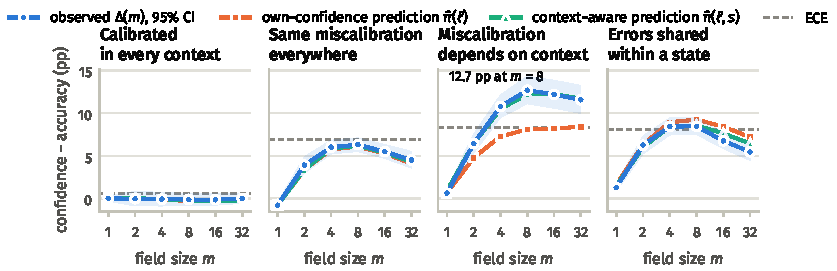
\includegraphics[width=0.88\linewidth]{t0_scenarios}\par
  \vspace{1.5mm}\raggedright
  \begin{takeaway}
    \textbf{Why ECE is not enough.} When miscalibration depends on context, ECE is
    \pct{\TZeroECEContext}\pp but $\Delta(32) - \Delta(1) = \pct{\TZeroContrastContext}$\pp.
    Known weakness: the field-term estimator reads high (\pct{\TZeroFieldContext}\pp against a
    true \pct{\TZeroFieldTrueContext}\pp).
  \end{takeaway}
\end{frame}

% ================================================================ 9 C1 results: E1/E2 (placeholder)
\begin{frame}{C1 results: does winning make a token overconfident? (E1, E2)}
  \vspace{2mm}
  \begin{pending}{TUE 27 OCT}{Report-half analysis: \texttt{C3\_REPORT\_HALF\_OK=1 bash prereg/analysis\_commands.sh}
    at tag \texttt{prereg-v1} (8B arms: Abhiraj; 110M arms: Ojas). Macros: \texttt{results/c1/<Label>/macros.tex}, prefix \texttt{COne<Label>}.}
    \begin{stubs}
      \item Figure: $\Delta(m)$ against field size $m$, one panel per model (LLaDA-8B, Dream-7B,
            110M), primary arms \texttt{uniform} and \texttt{decoder:topk\_conf:k4}.
      \item Table: $\Delta(32) - \Delta(1)$ with 95\% interval and the Holm verdict per arm
            (models $\times$ datasets); ECE beside it.
      \item E2: field term at $m = 32$ from the own and the context-aware calibrator.
      \item One-line answer to H1 and H2, with the null stated plainly if that is what we get.
    \end{stubs}
  \end{pending}
  \note{Pass 2: replace the box with the Delta(m) figure from results/c1/*/ and a table of
  COne<Label> macros. Backup: knots 5 and 13 panel, contamination-clean arms, Eq. 2/3
  beta\_z and gamma\_k.}
\end{frame}

% ================================================================ 10 C1 results: E3/T8 (placeholder)
\begin{frame}{C1 results: decoder states, tasks and controls (E3, T8)}
  \vspace{2mm}
  \begin{pending}{TUE 27 OCT}{Same run: \texttt{scripts/analyze\_e3.py} (prefix \texttt{EThree<Label>})
    and \texttt{scripts/run\_controls.py} (prefix \texttt{TEight<Label>}).}
    \begin{stubs}
      \item E3: decoder-induced states against matched-uniform states at equal confidence,
            per model; answer to H3.
      \item Instruct models on GSM8K and MBPP: is the committed-token gap larger on tasks
            than on web text?
      \item T8 ablation table: position, token type, per-step temperature; LLaDA-8B-Base
            4-bit against fp16 on the precision subset.
      \item Time-split arms: the same contrasts on text the 8B models cannot have seen.
    \end{stubs}
  \end{pending}
\end{frame}

% ================================================================ 11 C2 probe
\begin{frame}{C2: a JSON probe where the true joint $p^{*}$ is known}
  \framesubtitle{Our 110M model, fine-tuned on the probe; both terms computed exactly at every decoding step}
  \vspace{1mm}
  \begin{columns}[T,onlytextwidth]
    \begin{column}{0.5\textwidth}
      \begin{itemize}\footnotesize
        \item \textbf{Instances}: the simple fields of \VivaProbeSchemas{} SchemaStore schemas,
              \VivaProbeFieldsMin–\VivaProbeFieldsMax{} per schema, single-token values with
              seeded Dirichlet marginals.
        \item \textbf{Dependency knob $\rho$}: fields are paired. With probability $\rho$,
              stated in a marker at the start, the follower is a fixed function of its leader;
              otherwise an independent draw. So $p^{*}$ is exact.
        \item \textbf{Model}: our 110M fine-tuned on \VivaProbeTrainK k instances; evaluated
              on \CTwoProbeNInstances{} (\CTwoProbeNInstancesPerRho{} per $\rho$).
        \item \textbf{Decoding}: all values masked; each step a rule picks $k$ fields, the most
              confident or at random, and we fill them with the true values.
        \item \textbf{Check}: \A + \B equals the directly computed KL; largest error
              \CTwoIdentityMaxErrAll{} nats (bar \CTwoIdentityTol).
      \end{itemize}
    \end{column}
    \begin{column}{0.46\textwidth}
      \vspace{1mm}
      % instance text: artifacts/probe/eval_instances.jsonl, schema "tsd", rho = 1; values masked
      \begin{panel}[colback=plane, colframe=plane]
        {\color{ink2}\scriptsize one evaluation instance ($\rho = 1$), values masked}\par\vspace{1mm}
        \ttfamily\scriptsize
        \{{\color{accentdark}"\_rho":"1.00"},\\
        \hspace*{2mm}"bundle":{\color{muted}[M]}, "path":{\color{muted}[M]},\\
        \hspace*{2mm}"ref":{\color{muted}[M]}, "repo":{\color{muted}[M]},\\
        \hspace*{2mm}"stats":{\color{muted}[M]}, "version":{\color{muted}[M]}\}
      \end{panel}
      \vspace{1.5mm}
      \begin{panel}
        \paneltitle{Per step, for the committed set $S$}
        \A $= \sum_{i\in S} H(p^{*}_i) - H(p^{*}_S)$: zero unless a leader and its follower
        are committed together.\par\vspace{0.6mm}
        \B $= \sum_{i\in S}\mathrm{KL}(p^{*}_i \,\|\, p_{\theta,i})$: mass off the allowed values
        counts against \B.\par\vspace{0.6mm}
        Summed over steps, per field, bootstrapped over instances.
      \end{panel}
    \end{column}
  \end{columns}
  % rho grid {0, .25, .5, .75, 1}: artifacts/probe/spec.json (rhos); k {1, 2, 4, 8}: T9 grid.
\end{frame}

% ================================================================ 12 C2 crossover
\begin{frame}{C2: dependency overtakes estimation only at high $\rho$ and $k$}
  \vspace{0.5mm}
  \begin{columns}[T,onlytextwidth]
    \begin{column}{0.53\textwidth}
      \centering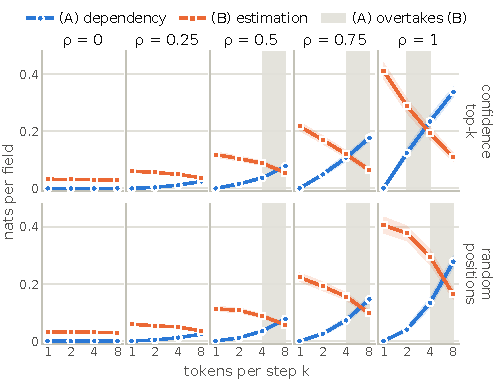
\includegraphics[height=58mm]{c2_crossover_ft110m-v3-visible}
    \end{column}
    \begin{column}{0.45\textwidth}
      \vspace{1mm}
      \begin{itemize}\footnotesize
        \item \A is zero at $k = 1$ and at $\rho = 0$, and grows with both.
        \item For $\rho \ge \CTwoConfCrossRhoMin$, \A overtakes \B at
              $k = \CTwoRandCrossKatRhoOne$; at $\rho = 1$ under confidence top-$k$ already at
              $k = \CTwoConfCrossKatRhoOne$. Each crossover is also where the 95\% interval of
              \A$-$\B clears zero.
        \item For $\rho \le 0.25$, \B dominates up to $k = 8$.
      \end{itemize}
      \vspace{1.5mm}
      \begin{panel}[colback=wash, colframe=wash]
        \paneltitle{$\rho = 1$, $k = 8$, confidence top-$k$}
        \A \CTwoConfAatRhoOneKEight{} \ci{\CTwoConfAatRhoOneKEightLo, \CTwoConfAatRhoOneKEightHi}
        and \B \CTwoConfBatRhoOneKEight{} \ci{\CTwoConfBatRhoOneKEightLo, \CTwoConfBatRhoOneKEightHi}
        nats per field: \A is \CTwoConfShareAatRhoOneKEight\% of the total.
      \end{panel}
      \src{Main model: the fine-tune that never saw the $\rho$ marker masked (choice in the
      backup). \CTwoProbeNBoot{} bootstrap resamples over instances.}
    \end{column}
  \end{columns}
\end{frame}

% ================================================================ 13 C2 corrections
\begin{frame}{C2: three findings that correct our plan}
  \vspace{1mm}
  \begin{columns}[T,onlytextwidth]
    \begin{column}{0.5\textwidth}
      \begin{panel}[fontupper=\scriptsize, before skip=0pt, after skip=1.2mm]
        \paneltitle{1 · Confidence selection raises \A, not \B}
        {\color{muted}Planned: ranking on noisy confidences inflates \B.}\par
        Where \B is higher than at random, the intervals overlap. \A rises instead
        ($\rho = 1$, $k = 2$): \CTwoConfAatRhoOneKTwo{} \ci{\CTwoConfAatRhoOneKTwoLo,
        \CTwoConfAatRhoOneKTwoHi} against \CTwoRandAatRhoOneKTwo{} \ci{\CTwoRandAatRhoOneKTwoLo,
        \CTwoRandAatRhoOneKTwoHi} at random.
      \end{panel}
      \begin{panel}[fontupper=\scriptsize, before skip=0pt, after skip=1.2mm]
        \paneltitle{2 · \B depends on $\rho$}
        {\color{muted}Planned: $\rho$ moves only \A.}\par
        At $k = 1$, \B rises from \CTwoConfBatRhoZeroKOne{} at $\rho = 0$ to
        \CTwoConfBatRhoOneKOne{} at $\rho = 1$: the model reads the marker only in part.
      \end{panel}
      \begin{panel}[fontupper=\scriptsize, before skip=0pt, after skip=1.2mm]
        \paneltitle{3 · \A and \B trade off along $k$}
        At $\rho = 1$, from $k = 1$ to $8$, \B falls from \CTwoConfBatRhoOneKOne{} to
        \CTwoConfBatRhoOneKEight{} while \A rises from 0 to \CTwoConfAatRhoOneKEight: a
        follower decoded with its leader shows its error as \A, not \B.
      \end{panel}
    \end{column}
    \begin{column}{0.47\textwidth}
      \centering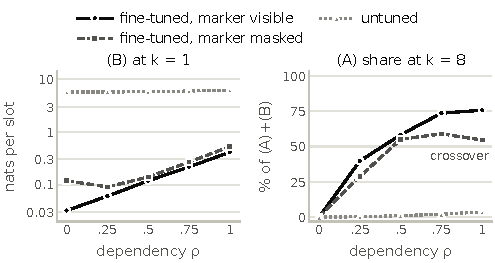
\includegraphics[width=\linewidth]{c2_untuned_vs_tuned}\par
      \vspace{1mm}\raggedright
      \begin{itemize}\footnotesize
        \item Without fine-tuning, \B dominates everywhere: \A is at most
              \CTwoUntunedConfShareAMax\% of the total.
        \item The ranking commits leaders together with their followers more often than
              chance, which brings the crossover forward.
      \end{itemize}
    \end{column}
  \end{columns}
\end{frame}

% ================================================================ 14 C2 real text
\begin{frame}{C2 on real text: the dependency proxy is near zero}
  \framesubtitle{\CTwoTTenNDocs{} fit-half FineWeb-Edu documents, one state per mask rate; the proxy is first checked on the probe}
  \vspace{0.5mm}
  \begin{columns}[T,onlytextwidth]
    \begin{column}{0.42\textwidth}
      \paneltitle{Proxies}
      {\scriptsize\raggedright
      For \A: \textbf{parallel--sequential disagreement}, the fraction of the $k$ most
      confident positions whose token changes when committed one at a time rather than in one
      pass. For \B: the gap $\Delta = c - a$ and the cross-entropy (CE) of the true token.\par}
      \vspace{1.5mm}
      \paneltitle{On the probe, it tracks \A weakly}
      {\scriptsize\raggedright
      Spearman with the exact \A over the \CTwoTTenProbeNCells{} confidence cells with
      $k \ge 2$: \CTwoTTenProbeSpearman{} \ci{\CTwoTTenProbeSpearmanLo,
      \CTwoTTenProbeSpearmanHi}; \CTwoTTenAltProbeSpearman{} for the other fine-tune. It rises
      with $k$, barely with $\rho$: at $k = 8$, \CTwoTTenProbeDisatRhoZeroKEight{} at
      $\rho = 0$, where \A is zero, and \CTwoTTenProbeDisatRhoOneKEight{} at $\rho = 1$.\par}
    \end{column}
    \begin{column}{0.55\textwidth}
      \scriptsize
      \setlength{\tabcolsep}{4pt}
      \renewcommand{\arraystretch}{1.12}
      \arrayrulecolor{base}
      % per_k_rates_below_1: mask rates 0.1-0.9 (rate 1 is one shared all-[MASK] state; backup)
      \begin{tabular}{@{}l l l@{}}
        \toprule
        {\color{ink2}mask rates 0.1–0.9} & {\color{ink2}110M (fp32)} & {\color{ink2}LLaDA-8B Base (fp16)} \\
        \midrule
        disagreement, $k = 4$ & \CTwoTTenDisKFour & \CTwoTTenLladaDisKFour \\
        disagreement, $k = 8$ & \CTwoTTenDisKEight & \CTwoTTenLladaDisKEight \\
        CE (nats), $k = 1 \rightarrow 8$ & \CTwoTTenCEKOne{} $\rightarrow$ \CTwoTTenCEKEight
          & \CTwoTTenLladaCEKOne{} $\rightarrow$ \CTwoTTenLladaCEKEight \\
        $\Delta$, $k = 1$ & \CTwoTTenDeltaKOne{} \ci{\CTwoTTenDeltaKOneLo, \CTwoTTenDeltaKOneHi}
          & \CTwoTTenLladaDeltaKOne{} \ci{\CTwoTTenLladaDeltaKOneLo, \CTwoTTenLladaDeltaKOneHi} \\
        $\Delta$, $k = 8$ & \CTwoTTenDeltaKEight{} \ci{\CTwoTTenDeltaKEightLo, \CTwoTTenDeltaKEightHi}
          & \CTwoTTenLladaDeltaKEight{} \ci{\CTwoTTenLladaDeltaKEightLo, \CTwoTTenLladaDeltaKEightHi} \\
        \bottomrule
      \end{tabular}
      \par\vspace{0.8mm}
      \fnote{CE includes the text's own entropy, and lower ranks are harder positions.}
      \vspace{1.5mm}
      \begin{takeaway}[fontupper=\scriptsize]
        At 2–8 tokens per step, real text looks like the probe's \textbf{low-$\rho$ regime,
        where \B dominates}. But the proxy sees only dependence the model has learned:
        near-zero disagreement does not show that \A is small.
      \end{takeaway}
    \end{column}
  \end{columns}
\end{frame}

% ================================================================ 15 C3 (placeholder)
\begin{frame}{C3: a recalibrated commit rule against six decoders}
  \vspace{2mm}
  \begin{pending}{THU 29 OCT}{T11 (the C3a policy and its calibrator, \texttt{artifacts/c3/}) and the T12
    sweep (Parth). Macros from the T12 scoring outputs.}
    \begin{stubs}
      \item C3a: commit every masked position in the active block whose recalibrated
            confidence clears $1 - \alpha$, and at least one. Calibrator fitted on the fit half
            of the LLaDA-8B-Instruct GSM8K and MBPP traces, then frozen.
      \item Matched-speed table: accuracy against tokens per step for top-$k$, the Fast-dLLM
            threshold, entropy-bounded, margin, KLASS, PC-Sampler and C3a, on the GSM8K and
            MBPP report halves; wall-clock beside it.
      \item Sanity row: top-$k$ and the threshold decoder against their published numbers.
      \item The answer in one line, including ``no gain at matched speed'' if that is the result.
    \end{stubs}
  \end{pending}
  \note{T12 settings (final-plan.md, Parth items 3-5): LLaDA-8B-Instruct free-running through
  c3/decode/loop.py, generation length 256, block 32, greedy, one seed, three speeds per
  decoder. If T12 is not done at the Fri 30 freeze, this slide becomes "C3: future work".}
\end{frame}

% ================================================================ 16 summary
\begin{frame}{Summary}
  \vspace{2mm}
  \begin{columns}[T,onlytextwidth]
    \begin{column}{0.485\textwidth}
      \begin{panel}[height=25mm]
        \paneltitle{1 · Theory}
        Selection alone cannot bias a calibrated posterior (Proposition 1). Any bias lives in
        the field term (Proposition 2), which the instrument measures and which T0 shows it
        can see where ECE cannot.
      \end{panel}
      \vspace{1.5mm}
      \begin{panel}[height=25mm, colback=wash, colframe=accent!40]
        \paneltitle{2 · C1 audit}
        {\color{ink2}Placeholder: the answers to H1–H3 on three model families, from the
        report half (Tue 27).}
      \end{panel}
    \end{column}
    \begin{column}{0.485\textwidth}
      \begin{panel}[height=25mm]
        \paneltitle{3 · C2: (A) and (B) separated}
        On the probe, \A overtakes \B only for $\rho \ge \CTwoConfCrossRhoMin$ and larger $k$;
        confidence selection raises \A, not \B. On real text at 2–8 tokens per step, the
        \A proxy is near zero: the \B-dominated regime.
      \end{panel}
      \vspace{1.5mm}
      \begin{panel}[height=25mm, colback=wash, colframe=accent!40]
        \paneltitle{4 · C3 decoding}
        {\color{ink2}Placeholder: C3a against six decoders at matched tokens per step
        (Thu 29).}
      \end{panel}
    \end{column}
  \end{columns}
\end{frame}

% ================================================================ 17 limitations
\begin{frame}{What we got wrong, and the limits of these results}
  \vspace{2mm}
  \begin{columns}[T,onlytextwidth]
    \begin{column}{0.485\textwidth}
      \begin{panel}[height=56mm]
        \paneltitle{Claims we withdrew}
        \begin{itemize}\scriptsize
          \item Heteroskedastic noise alone makes winners overconfident (proposal):
                false, Proposition 1.
          \item Selection on confidence inflates \B (proposal, mid report): on the probe it
                raises \A instead.
          \item $\rho$ moves only \A (plan v2): \B rises with $\rho$ too.
          \item C2 on an 8B model (plan v2): not run. The probe results are for our 110M only.
          \item Real-text C2 as identified contrasts (mid deck): they are proxies, with a
                direction but no split in nats.
        \end{itemize}
      \end{panel}
    \end{column}
    \begin{column}{0.485\textwidth}
      \begin{panel}[height=56mm]
        \paneltitle{Limits}
        \begin{itemize}\scriptsize
          \item C2's exact values hold for one synthetic distribution and one 110M model.
          \item The main probe model was chosen by a fallback (lower validation NELBO) after
                neither fine-tune met a bar that was itself written down with the results:
                \textbf{not pre-registered}. The other model's crossovers are in the backup.
          \item The disagreement proxy tracks \A weakly, and mostly through $k$.
          \item 8B models in fp16, not bfloat16 (no bfloat16 on our GPUs); E3 for top-$k$
                decoders only (\texttt{prereg/deviations.md}).
          \item {\color{ink2}C1 and C3 limits: pass 2.}
        \end{itemize}
      \end{panel}
    \end{column}
  \end{columns}
\end{frame}

% ================================================================ 18 thanks
\begin{frame}[c,plain]
  \hspace*{4mm}\begin{minipage}{0.86\linewidth}\raggedright
    {\fontsize{24}{28}\selectfont\firasemibold Thank you. Questions?}\par
    \vspace{3mm}
    {\color{accent}\rule{14mm}{1.6pt}}\par
    \vspace{4mm}
    \small\color{ink2}
    \begin{tabular}{@{}ll@{}}
      Code              & github.com/abhirajratna/ANLP-Project \\
      Weights \& Biases & wandb.ai/ANLP-project/c3-dllm-calibration \\
      Hugging Face      & huggingface.co/ANLP-project \\
      Paper             & DuckDuckDuckGoose-Final.zip \\
    \end{tabular}
  \end{minipage}
\end{frame}

% ================================================================ backup
\appendix

\begin{frame}{Backup: proofs}
  \framesubtitle{$W_i$: the event that $i \in P$ wins, $i = \arg\max_{j\in P}\ell_j$; ties broken by independent randomness $U$}
  \vspace{1.5mm}
  \footnotesize
  \begin{columns}[T,onlytextwidth]
    \begin{column}{0.485\textwidth}\raggedright
      \paneltitle{Proposition 1}
      Suppose, given $s$, each pair $(\ell_i, a_i)$ is independent of
      $\ell_{-i} = (\ell_j)_{j \in M\setminus\{i\}}$. Let $Z = (\ell_i, s)$ and
      $Y = (\ell_{-i}, P, U)$.\par\vspace{1mm}
      Given $s$, $(\ell_i, a_i) \perp \ell_{-i}$ and $(P, U) \perp (\ell_j, a_j)_{j\in M}$, so
      $(\ell_i, a_i) \perp Y \mid s$, and by weak union $a_i \perp Y \mid Z$, i.e.\
      $\mathbb{E}[a_i \mid Y, Z] = \pi(\ell_i, s)$.\par\vspace{1mm}
      $W_i$ is determined by $(Y, Z)$, so for every bounded measurable $h$
      \[
        \mathbb{E}[a_i h(Z) \mathbb{1}_{W_i}] = \mathbb{E}[\pi(\ell_i, s) h(Z) \mathbb{1}_{W_i}].
      \]
      Dividing by $\Pr(W_i) > 0$ gives $\mathbb{E}[a_i \mid Z, W_i] = \pi(\ell_i, s)$ a.s.
    \end{column}
    \begin{column}{0.485\textwidth}\raggedright
      \paneltitle{Proposition 2}
      Exactly one $W_i$ holds. Applying the display with $h \equiv 1$, summing over $i$ and
      averaging over $s$:
      \[
        \mathbb{E}_m[a] = \textstyle\sum_i \mathbb{E}_m[a_i \mathbb{1}_{W_i}]
        = \textstyle\sum_i \mathbb{E}_m[\pi(\ell_i, s)\mathbb{1}_{W_i}]
        = \mathbb{E}_m[\pi(\ell, s)],
      \]
      so $\Delta(m) = \mathbb{E}_m[\sigma(\ell) - \pi(\ell, s)]$; add and subtract
      $\pi(\ell)$.\par\vspace{1mm}
      At $m = 1$, $\mathbb{E}_1[\pi(\ell)] = \mathbb{E}_1[a]$ by the tower property and
      $\mathbb{E}_1[\pi(\ell, s)] = \mathbb{E}_1[a]$ by the display, so the field term is 0.
    \end{column}
  \end{columns}
\end{frame}

\begin{frame}{Backup: how the main probe model was chosen}
  \framesubtitle{Recorded in \texttt{artifacts/probe/main\_variant.json}}
  \begin{columns}[T,onlytextwidth]
    \begin{column}{0.5\textwidth}
      \footnotesize
      \renewcommand{\arraystretch}{1.12}
      \arrayrulecolor{base}
      \scriptsize
      \begin{tabularx}{\linewidth}{@{}L r r@{}}
        \toprule
        & {\color{ink2}\CTwoVariant} & {\color{ink2}\CTwoAltVariant} \\
        \midrule
        $\rho$ marker in fine-tuning & never masked & masked \\
        Fine-tuning tokens (M) & \CTwoFtTokensM & \CTwoAltFtTokensM \\
        Marker effect on copy & \CTwoMarkerEffect & \CTwoAltMarkerEffect \\
        Val.\ NELBO (nats/tok.) & \CTwoValNelbo & \CTwoAltValNelbo \\
        First $k$ with \A $>$ \B ($\rho{=}1$) & \CTwoConfCrossKatRhoOne & \CTwoAltConfCrossKatRhoOne \\
        \bottomrule
      \end{tabularx}
      \par\vspace{1mm}
      \begin{itemize}\scriptsize
        \item The bar for the main result, a marker effect of \CTwoMarkerBar, was first written
              down \emph{with} these results. Neither model meets it.
        \item The fallback, the lower validation NELBO, is stated as a rule in no committed
              file; it was applied when the choice was made. \textbf{Not pre-registered.}
        \item The other model crosses over at $k = \CTwoAltConfCrossKatRhoOne$ for every
              $\rho \ge \CTwoAltConfCrossRhoMin$ under both rules: the qualitative picture
              holds.
      \end{itemize}
    \end{column}
    \begin{column}{0.47\textwidth}
      \centering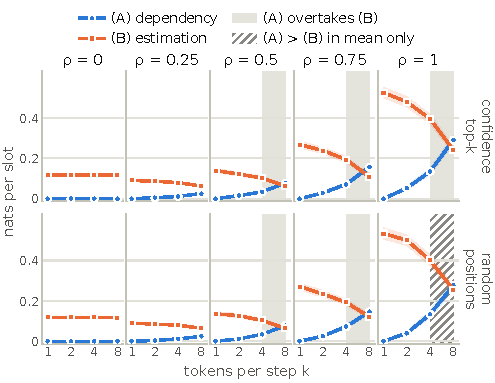
\includegraphics[height=48mm]{c2_crossover_ft110m-v3}\par
      \fnote{As the main figure, for \CTwoAltVariant. Hatched: \A $>$ \B in mean only.}
    \end{column}
  \end{columns}
\end{frame}

\begin{frame}{Backup: disagreement by mask rate (T10)}
  \framesubtitle{Disagreement at $k = 8$ per mask rate; one state per document per rate}
  \vspace{2mm}
  \centering\footnotesize
  \renewcommand{\arraystretch}{1.1}
  \arrayrulecolor{base}
  % mask rates 0.1 ... 1: config.rates in both T10 JSONs
  \begin{tabular}{@{}l r r r r r r r r r r@{}}
    \toprule
    {\color{ink2}Mask rate} & 0.1 & 0.2 & 0.3 & 0.4 & 0.5 & 0.6 & 0.7 & 0.8 & 0.9 & 1 \\
    \midrule
    110M & \CTwoTTenDisKEightRatePtOne & \CTwoTTenDisKEightRatePtTwo & \CTwoTTenDisKEightRatePtThree
      & \CTwoTTenDisKEightRatePtFour & \CTwoTTenDisKEightRatePtFive & \CTwoTTenDisKEightRatePtSix
      & \CTwoTTenDisKEightRatePtSeven & \CTwoTTenDisKEightRatePtEight & \CTwoTTenDisKEightRatePtNine
      & \CTwoTTenDisKEightRateOne \\
    LLaDA-8B-Base & \CTwoTTenLladaDisKEightRatePtOne & \CTwoTTenLladaDisKEightRatePtTwo & \CTwoTTenLladaDisKEightRatePtThree
      & \CTwoTTenLladaDisKEightRatePtFour & \CTwoTTenLladaDisKEightRatePtFive & \CTwoTTenLladaDisKEightRatePtSix
      & \CTwoTTenLladaDisKEightRatePtSeven & \CTwoTTenLladaDisKEightRatePtEight & \CTwoTTenLladaDisKEightRatePtNine
      & \CTwoTTenLladaDisKEightRateOne \\
    \bottomrule
  \end{tabular}
  \par\vspace{4mm}\raggedright
  \begin{itemize}\footnotesize
    \item At rate 1 every input is the same all-\texttt{[MASK]} sequence. That one state gives
          the 110M model nearly all of its disagreement (\CTwoTTenDisAllRatesKEight{} at $k = 8$
          over all ten rates); LLaDA does not disagree there. The main slide reads rates
          0.1–0.9.
    \item Documents under 256 tokens are skipped (a deviation from the plan); at least
          \CTwoTTenMinMasked{} masked positions per state; \CTwoTTenNBoot{} document-bootstrap
          resamples.
  \end{itemize}
\end{frame}

\begin{frame}{Backup: data, contamination and our 110M model}
  \vspace{1.5mm}
  \begin{columns}[T,onlytextwidth]
    \begin{column}{0.5\textwidth}
      \begin{itemize}\footnotesize
        \item \textbf{\VivaCorpusDocs{} calibration documents}, reservoir-sampled from
              FineWeb-Edu with a fixed seed and excluded from our 110M's training stream;
              \VivaNFit{} fit / \VivaNReport{} report.
        \item \textbf{Tasks}: GSM8K and MBPP test sets, split 50/50 the same way, as
              teacher-forced documents.
        \item \textbf{Contamination screen (T4)}: prompt with \VivaLladaContamPrefix{} tokens,
              continue greedily, flag a verbatim run $\ge \VivaContamThreshold$ tokens.
              Flagged: \VivaLladaContamFlagged/\VivaLladaContamDocs{} (LLaDA),
              \VivaDreamContamFlagged/\VivaDreamContamDocs{} (Dream); the 8B arms are also
              analysed without them.
        \item \textbf{Time-split set}: text written after the 8B models were trained.
      \end{itemize}
    \end{column}
    \begin{column}{0.46\textwidth}
      \footnotesize
      \renewcommand{\arraystretch}{1.08}
      \arrayrulecolor{base}
      \begin{tabularx}{\linewidth}{@{}l L@{}}
        \toprule
        Model     & bidirectional transformer: \VivaMdlmLayers{} layers, width \VivaMdlmWidth,
                    \VivaMdlmHeads{} heads; sequence length \VivaMdlmSeqLen \\
        Objective & MDLM (weighted masked cross-entropy), GPT-2 BPE + [MASK] \\
        Training  & \VivaMdlmSteps{} steps, \VivaMdlmTokensB{}B tokens of FineWeb-Edu \\
        \bottomrule
      \end{tabularx}
      \par\vspace{2mm}
      \begin{columns}[T,onlytextwidth]
        \begin{column}{0.48\textwidth}
          \begin{panel}[colback=wash, colframe=wash, height=22mm]
            \stat{\VivaMdlmPplBound}{perplexity \emph{bound} on the \VivaMdlmEvalDocs{} held-out
              docs \ci{\VivaMdlmPplBoundLo, \VivaMdlmPplBoundHi}}
          \end{panel}
        \end{column}
        \begin{column}{0.48\textwidth}
          \begin{panel}[height=22mm]
            \stat{\VivaGptTwoPpl}{GPT-2 small, \emph{exact} perplexity, same docs
              \ci{\VivaGptTwoPplLo, \VivaGptTwoPplHi}}
          \end{panel}
        \end{column}
      \end{columns}
      \fnote{MDLM gives only an upper bound, and GPT-2 saw other data with far more compute.}
    \end{column}
  \end{columns}
\end{frame}

\begin{frame}{Backup: references}
  \vspace{1.5mm}
  \scriptsize
  \setlength{\parskip}{2.4pt}
  \raggedright\color{ink2}
  Andrews, Kitagawa \& McCloskey (2024). Inference on winners. \emph{Quarterly Journal of Economics} 139(1).\par
  Azangulov et al.\ (2026). Parallel sampling from masked diffusion models via conditional independence. \emph{ICLR}.\par
  Ben-Hamu et al.\ (2025). Accelerated sampling from masked diffusion models via entropy bounded unmasking. \emph{NeurIPS}.\par
  Chang et al.\ (2022). MaskGIT: masked generative image transformer. \emph{CVPR}.\par
  Cobbe et al.\ (2021). Training verifiers to solve math word problems. arXiv:2110.14168.\par
  Efron (2011). Tweedie's formula and selection bias. \emph{JASA} 106(496).\par
  Guo et al.\ (2017). On calibration of modern neural networks. \emph{ICML}.\par
  Kang et al.\ (2026). ParallelBench: understanding the trade-offs of parallel decoding in diffusion LLMs. \emph{ICLR}.\par
  Kim et al.\ (2026). DAPD: dependency-aware parallel decoding via attention for diffusion LLMs. \emph{ICML}.\par
  Nie et al.\ (2025). Large language diffusion models. \emph{NeurIPS}.\par
  Penedo et al.\ (2024). The FineWeb datasets: decanting the web for the finest text data at scale. arXiv:2406.17557.\par
  Ringel, Ali \& Romano (2026). Dependency-guided parallel decoding in discrete diffusion language models. arXiv:2604.02560.\par
  Sahoo et al.\ (2024). Simple and effective masked diffusion language models. \emph{NeurIPS}.\par
  SchemaStore contributors (2026). SchemaStore. github.com/SchemaStore/schemastore.\par
  Tang et al.\ (2026). Is your diffusion sampler actually correct? \emph{ICML}.\par
  Wu et al.\ (2025). Fast-dLLM: training-free acceleration of diffusion LLM. arXiv:2505.22618.\par
\end{frame}

\end{document}
